% ============================================================
%  The Particle Model — Lesson Booklet (one section per lesson: A Reading · B Theory · C Practice · D Above level)
%  Year 7 (Year 8 extension)  |  Victorian Curriculum F–10 Version 2.0
%  Compile with: xelatex three times, then python3 fill.py Particle_Model_Lesson_Booklet_Yr7
% ============================================================
\documentclass[11pt,a5paper,twoside]{article}

% ── Fonts (compile with LuaLaTeX) ────────────────────────────────────────────
\usepackage{fontspec}
% Bundled fonts (in ./fonts/) so the document compiles anywhere with XeLaTeX/LuaLaTeX
\setmainfont{Lato}[                   % body — humanist sans (stands in for deck's Inter)
  Path=../fonts/, Extension=.ttf, Ligatures=TeX,
  UprightFont=Lato-Regular, ItalicFont=Lato-Italic,
  BoldFont=Lato-Bold, BoldItalicFont=Lato-BoldItalic ]
\newfontfamily\headingfont{Poppins}[  % display/headings — matches the slide decks
  Path=../fonts/, Extension=.ttf, Ligatures=TeX,
  UprightFont=Poppins-Regular, ItalicFont=Poppins-Italic,
  BoldFont=Poppins-Bold, BoldItalicFont=Poppins-BoldItalic ]
\setlength{\headheight}{22pt}

\usepackage[protrusion=true,expansion=false]{microtype}
\usepackage[a5paper, inner=17mm, outer=13mm, top=19mm, bottom=17mm, headheight=14pt, headsep=4mm, footskip=8mm]{geometry}
\usepackage{xcolor}
\usepackage{tikz}
\usetikzlibrary{arrows.meta, shapes.geometric, calc, positioning, decorations.pathreplacing}
\usepackage{tcolorbox}
\tcbuselibrary{skins, breakable, raster}
\usepackage{fancyhdr}
\usepackage{titlesec}
\usepackage{enumitem}
\usepackage{booktabs}
\usepackage{tabularx}
\usepackage{array}
\usepackage{colortbl}
\usepackage{multicol}
\usepackage{amsmath}
\usepackage{needspace}
% TikZ diagram macros are embedded below (just before \begin{document}) for easy editing.
\usepackage{longtable}
\usepackage{graphicx}
\usepackage{lastpage}
\usepackage{calc}
\usepackage{mdframed}
\usepackage{setspace}
\usepackage{ragged2e}
% PDF bookmarks: one per lesson (made in \sectiondiv) plus the cover and
% contents, and links from the contents table to each lesson.
% implicit=false: hyperref adds no anchors of its own (an anchor on each
% list item nudged lists down 1.5 mm, which would undo the page fill).
% hidelinks keeps the links invisible, so the printed pages are unchanged.
\usepackage[implicit=false, hidelinks,
  pdftitle={The Particle Model — Lesson Booklet (A5)},
  pdfsubject={Years 7–8 Science, Victorian Curriculum F–10 v2.0}]{hyperref}
\usepackage{bookmark} % writes the outline itself, which implicit=false switches off in hyperref
% hyperref 7.01 with implicit=false leaves \Hy@PageAnchorSlide undefined, which
% throws at \end{document} and stops fill.py (it builds with -halt-on-error).
\makeatletter\providecommand\Hy@PageAnchorSlide{}\makeatother

% ── Colour Palette ───────────────────────────────────────────────────────────
% Remapped to the slide-deck palette (names kept so body + diagrams cascade)
\definecolor{NavyBlue}   {HTML}{16305C}
\definecolor{MidBlue}    {HTML}{2E6FE0}
\definecolor{LightBlue}  {HTML}{E8F1FF}
\definecolor{TealGreen}  {HTML}{0F6E63}
\definecolor{LightGreen} {HTML}{E0F7F3}
\definecolor{GoldDark}   {HTML}{C77F12}
\definecolor{GoldLight}  {HTML}{FFF3DC}
\definecolor{PurpleDark} {HTML}{5B3FC0}
\definecolor{PurpleLight}{HTML}{EFE9FF}
\definecolor{OrangeDark} {HTML}{C9483D}
\definecolor{OrangeLight}{HTML}{FFE9E6}
\definecolor{MidGrey}    {HTML}{AEBED4}
\definecolor{LightGrey}  {HTML}{F2F5FA}
\definecolor{DarkGrey}   {HTML}{3A4759}
\definecolor{TableHead}  {HTML}{16305C}
\definecolor{RowAlt}     {HTML}{EEF4FF}
% Bright accent tints (deck) for bars, rules and chips
\definecolor{Blue}   {HTML}{2E6FE0}
\definecolor{Teal}   {HTML}{18A999}
\definecolor{Amber}  {HTML}{F5A623}
\definecolor{Coral}  {HTML}{FF6B5E}
\definecolor{Violet} {HTML}{7C5CE0}
\definecolor{Sky}    {HTML}{4DA3FF}
\definecolor{Ink}    {HTML}{16223A}
\definecolor{Line}   {HTML}{DDE5F0}
\definecolor{Paper}  {HTML}{FBFCFE}

% ── Page Style ───────────────────────────────────────────────────────────────
\pagestyle{fancy}
\fancyhf{}
\renewcommand{\headrulewidth}{0.4pt}
\renewcommand{\headrule}{\hbox to\headwidth{\color{NavyBlue}\leaders\hrule height \headrulewidth\hfill}}
\fancyhead[L]{\headingfont\small\color{NavyBlue}The Particle Model}
\fancyhead[R]{\headingfont\small\color{DarkGrey}Year 7 \textbar{} Victorian Curriculum F--10 v2.0}
\fancyfoot[C]{\headingfont\small\color{DarkGrey}\thepage\ \textbar{} \pageref{LastPage}}
\fancypagestyle{plain}{%
  \fancyhf{}
  \fancyfoot[C]{\headingfont\small\color{DarkGrey}\thepage\ \textbar{} \pageref{LastPage}}
  \renewcommand{\headrulewidth}{0pt}
}

% ── Section Formatting ───────────────────────────────────────────────────────
\titleformat{\section}
  {\headingfont\color{NavyBlue}\Large\bfseries}
  {}{0em}{}
  [{\color{Teal}\rule[0.6ex]{2.2em}{3pt}}{\color{Line}\rule[0.6ex]{\dimexpr\linewidth-2.2em\relax}{1pt}}]
\titlespacing{\section}{0pt}{18pt}{8pt}

\titleformat{\subsection}
  {\headingfont\color{MidBlue}\large\bfseries}
  {\thesubsection}{0.6em}{}
\titlespacing{\subsection}{0pt}{12pt}{4pt}

\titleformat{\subsubsection}
  {\headingfont\color{NavyBlue}\normalsize\bfseries}
  {}{0em}{}
\titlespacing{\subsubsection}{0pt}{8pt}{2pt}

% Deck-style eyebrow / kicker (optional use)
\newcommand{\kicker}[2][Teal]{%
  {\headingfont\bfseries\footnotesize\color{#1}%
   \textcolor{#1}{\rule[0.18ex]{1.6em}{2.2pt}}\hspace{0.5em}\MakeUppercase{#2}\par}%
  \vspace{2pt}}

% ── Custom tcolorbox Environments ────────────────────────────────────────────

% Section divider banner
\newtcolorbox{sectionbanner}[2]{
  enhanced, breakable=false,
  colback=NavyBlue, colframe=NavyBlue,
  fontupper=\color{white}\bfseries\large,
  left=4mm, right=4mm, top=3mm, bottom=3mm,
  title={\color{white}\Huge\bfseries #1},
  attach boxed title to top left={yshift=-2mm, xshift=4mm},
  boxed title style={colback=NavyBlue, colframe=NavyBlue},
  after upper={\par\smallskip\normalfont\normalsize\color{white!80!NavyBlue}\textit{#2}}
}

% Key info box (blue)
\newtcolorbox{infobox}[1]{
  breakable, arc=2.5mm, boxrule=0.5pt,
  colback=LightBlue, colframe=Blue!40,
  fonttitle=\headingfont\bfseries, coltitle=MidBlue,
  title={#1},
  left=4mm, right=3.5mm, top=2.5mm, bottom=2.5mm
}

% Scaffold box (yellow)
\newtcolorbox{scaffold}[1]{
  breakable, arc=2.5mm, boxrule=0.5pt,
  colback=GoldLight, colframe=Amber!40,
  fonttitle=\headingfont\bfseries, coltitle=GoldDark,
  title={#1},
  left=4mm, right=3.5mm, top=2.5mm, bottom=2.5mm
}

% Worked example box
\newtcolorbox{workedexbox}[1]{
  breakable, arc=2.5mm, boxrule=0.5pt,
  colback=white, colframe=Amber!50,
  fonttitle=\headingfont\bfseries, coltitle=GoldDark,
  title={#1},
  left=4mm, right=3.5mm, top=2.5mm, bottom=2.5mm
}
% Worked examples: \begin{workedex}{title} -> "Worked Example N.M --- title",
% auto-numbered per section and labelled we:N.M. Never type the number.
\newcounter{wenum}[section]
\renewcommand{\thewenum}{\thesection.\arabic{wenum}}
\newenvironment{workedex}[1]
  {\refstepcounter{wenum}\label{we:\thewenum}\begin{workedexbox}{Worked Example \thewenum\ --- #1}}
  {\end{workedexbox}}

% We do: straight after each worked example, a near-identical question the
% class works through together, with its own writing space. Numbered to
% match the worked example above it and labelled wd:N.M.
%   \begin{wedo}{title} question ... \answerbox{h} \end{wedo}
\newtcolorbox{wedobox}[1]{
  enhanced, breakable=false, arc=2.5mm, boxrule=0.5pt,
  colback=white, colframe=TealGreen!55,
  fonttitle=\headingfont\bfseries, coltitle=TealGreen!75!black,
  title={#1},
  left=4mm, right=3.5mm, top=2.5mm, bottom=2.5mm
}
\newenvironment{wedo}[1]
  {\par\needspace{9\baselineskip}\begin{wedobox}{We do \thewenum\ --- #1}\label{wd:\thewenum}\ignorespaces}
  {\end{wedobox}}

% Year 7 box (blue)
\newtcolorbox{yr7box}{
  breakable, arc=2.5mm, boxrule=0.5pt,
  colback=LightBlue, colframe=Blue!40,
  left=4mm, right=3.5mm, top=2.5mm, bottom=2.5mm
}

% Year 8 extension box (violet)
\newtcolorbox{yr8box}{
  breakable, arc=2.5mm, boxrule=0.5pt,
  colback=PurpleLight, colframe=Violet!40,
  left=4mm, right=3.5mm, top=2.5mm, bottom=2.5mm
}

% Answer lines box
\newcommand{\answerbox}[1]{%
  \begin{tcolorbox}[
    enhanced, breakable, arc=2mm,
    colback=Paper, colframe=Line,
    left=2mm, right=2mm, top=1mm, bottom=1mm,
    boxrule=1pt,
    height=#1
  ]
  \end{tcolorbox}%
}

% Experiment header
\newtcolorbox{expheader}[3]{
  breakable=false, arc=2.5mm,
  colback=RowAlt, colframe=Amber!50, boxrule=0.5pt,
  fonttitle=\headingfont\bfseries\large, coltitle=NavyBlue,
  title={Experiment #1: #2},
  left=4mm, right=3.5mm, top=2.5mm, bottom=2.5mm,
  after upper={\par\smallskip
    {\headingfont\bfseries\color{GoldDark}Aim:}\ \textit{#3}},
}

% Reading comprehension passage box (green)
\newtcolorbox{readingbox}[1]{
  breakable, arc=2.5mm, boxrule=0.5pt,
  colback=white, colframe=Teal!50,
  fonttitle=\headingfont\bfseries, coltitle=TealGreen,
  title={#1},
  left=4mm, right=3.5mm, top=2.5mm, bottom=2.5mm,
  fontupper=\normalsize
}

% Skill-builder box (for beginner scaffolding)
\newtcolorbox{skillbox}[1]{
  breakable, arc=2.5mm, boxrule=0.5pt,
  colback=RowAlt, colframe=Blue!40,
  fonttitle=\headingfont\bfseries, coltitle=MidBlue,
  title={#1},
  left=4mm, right=3.5mm, top=2.5mm, bottom=2.5mm
}

% ── Custom Commands ───────────────────────────────────────────────────────────

% Question: \question{marks}{text}  (marks can be empty)
% Numbered automatically as Q<section>.<n>, reset every section.
% Do NOT write numbers by hand.
\newcounter{qnum}[section]
\renewcommand{\theqnum}{\thesection.\arabic{qnum}}
\newcommand{\question}[2]{%
  \refstepcounter{qnum}%
  \needspace{3\baselineskip}%
  \medskip
  \noindent\label{q:\theqnum}\textbf{Q\theqnum}\ifx&#1&\else\ \textcolor{DarkGrey}{(#1 mark\ifnum#1=1\else s\fi)}\fi\quad #2%
  \medskip
}

% Inline marks note
\newcommand{\markscount}[1]{\hfill\textcolor{DarkGrey}{\textit{(#1 mark\ifnum#1=1\else s\fi)}}}

% ── Practice set counter and question macros ─────────────────────────────────
\newcounter{pqnum}
\newcommand{\practiceset}[1]{%
  \needspace{6\baselineskip}
  \setcounter{pqnum}{0}%
  \vspace{6pt}
  {\headingfont\bfseries\large\color{GoldDark} Practice Set --- #1}\\[-2pt]
  {\color{Amber}\rule{\linewidth}{1pt}}\\[2pt]
}
% \pq{question text}{working box height}
\newcommand{\pq}[2]{%
  \stepcounter{pqnum}%
  \needspace{4\baselineskip}
  \vspace{5pt}
  \noindent\textbf{\thepqnum.}\quad #1\par
  \vspace{2pt}
  \answerbox{#2}
}
% Two short questions side by side, each with its own box
\newcommand{\pqpair}[4]{%
  \needspace{4\baselineskip}
  \vspace{5pt}
  \noindent
  \begin{minipage}[t]{0.48\linewidth}
    \stepcounter{pqnum}\textbf{\thepqnum.}\quad #1\par\vspace{2pt}
    \begin{tcolorbox}[enhanced,arc=2mm,colback=Paper,colframe=Line,left=2mm,right=2mm,
      top=1mm,bottom=1mm,boxrule=1pt,height=#2]\end{tcolorbox}
  \end{minipage}\hfill
  \begin{minipage}[t]{0.48\linewidth}
    \stepcounter{pqnum}\textbf{\thepqnum.}\quad #3\par\vspace{2pt}
    \begin{tcolorbox}[enhanced,arc=2mm,colback=Paper,colframe=Line,left=2mm,right=2mm,
      top=1mm,bottom=1mm,boxrule=1pt,height=#4]\end{tcolorbox}
  \end{minipage}
}

% ── Comprehension question macro (compact, lined) ────────────────────────────
\newcounter{rcnum}
\newcommand{\rcreset}{\setcounter{rcnum}{0}}
\newcommand{\rcq}[2]{%
  \stepcounter{rcnum}%
  \needspace{3\baselineskip}
  \vspace{4pt}
  \noindent\textbf{C\thercnum.}\quad #1\par
  \vspace{2pt}
  \linedbox{#2}
}

% Section divider (big numbered banner): \sectiondiv{title}{summary}
%
% This IS the section: it steps the real section counter, so subsections,
% tasks, questions and figures inside it are numbered N.M automatically.
% Put \label{sec:N} straight after it. Never hand-type a section number.
\newcommand{\sectiondiv}[2]{%
  \needspace{5\baselineskip}%
  \refstepcounter{section}%
  % PDF bookmark for the lesson; its anchor, lesson.N.1, is what the contents table links to
  \pdfbookmark[1]{Lesson \thesection{} — #1}{lesson.\thesection}%
  \begin{tcolorbox}[
    enhanced, breakable=false, arc=3.5mm,
    colback=NavyBlue, colframe=NavyBlue, boxrule=0pt,
    sidebyside, sidebyside align=center,
    lefthand width=2.4cm,
    left=2mm, right=4mm, top=4mm, bottom=4mm
  ]
    \begin{center}
      {\headingfont\bfseries\color{white!35!NavyBlue}\fontsize{50}{50}\selectfont \thesection}
    \end{center}
    \tcblower
    {\headingfont\bfseries\color{white}\LARGE #1}\\[3pt]
    {\itshape\color{white!75!NavyBlue}\small #2}
  \end{tcolorbox}%
}

% Tasks: \task, \task[a] (part a of a NEW task), \taskpart{b} (next part
% of the same task), \exttask (Year 8 "Extension" — same counter).
% Numbered Task <section>.<n>, reset every section. Do NOT type numbers.
% Every task, question and figure also gets an automatic label
% (task:1.7b, q:2.4, fig:1.2, fig:E2.1) so page refs come from the .aux.
\newcounter{tasknum}[section]
\renewcommand{\thetasknum}{\thesection.\arabic{tasknum}}
\NewDocumentCommand{\task}{o}{\refstepcounter{tasknum}\label{task:\thetasknum\IfValueT{#1}{#1}}\textbf{Task \thetasknum\IfValueT{#1}{#1}}}
\newcommand{\taskpart}[1]{\label{task:\thetasknum#1}\textbf{Task \thetasknum#1}}
\newcommand{\exttask}{\refstepcounter{tasknum}\label{task:\thetasknum}\textbf{Extension \thetasknum}}

% Figure captions: \figcap[fig:label]{caption} -> "Figure N.M --- caption"
% \expfigcap{caption} -> "Figure EN.M" (experiment pages). Both auto-numbered.
\newcounter{fignum}[section]
\renewcommand{\thefignum}{\thesection.\arabic{fignum}}
\newcounter{expfignum}[section]
\renewcommand{\theexpfignum}{E\thesection.\arabic{expfignum}}
\newcommand{\figcap}[2][]{%
  \begin{center}
    \refstepcounter{fignum}\label{fig:\thefignum}\if\relax\detokenize{#1}\relax\else\label{#1}\fi
    \small\itshape\color{DarkGrey} Figure \thefignum\ --- #2
  \end{center}%
}
\newcommand{\expfigcap}[1]{%
  \begin{center}
    \refstepcounter{expfignum}\label{fig:\theexpfignum}%
    \small\itshape\color{DarkGrey} Figure \theexpfignum\ --- #1
  \end{center}%
}

% Diagram include
\newcommand{\diagramfig}[3]{%  {filename}{width fraction}{caption}
  \begin{center}
    \includegraphics[width=#2\linewidth]{#1}\\[4pt]
    \small\itshape\color{DarkGrey} #3
  \end{center}%
}

% Table column types
\newcolumntype{L}[1]{>{\RaggedRight\arraybackslash}p{#1}}
\newcolumntype{C}[1]{>{\Centering\arraybackslash}p{#1}}

% Table header colour
\newcommand{\thead}[1]{\cellcolor{TableHead}\color{white}\bfseries #1}
\newcommand{\talt}{\rowcolor{RowAlt}}
\newcommand{\tmid}{\rowcolor{MidGrey}}

% Inline year tags
\newcommand{\tagyr}[1]{%
  \tikz[baseline=-0.5ex]\node[
    rounded corners=2pt,
    fill=#1!20, draw=#1, text=#1,
    inner xsep=4pt, inner ysep=1pt,
    font=\scriptsize\bfseries
  ]{Yr #1 only};}

% Draw answer lines
\newcommand{\anslines}[1]{%
  \vspace{2pt}%
  \foreach \n in {1,...,#1}{%
    \par\noindent\rule{\linewidth}{0.3pt}\vspace{3pt}%
  }%
}

% ── Document ─────────────────────────────────────────────────────────────────
% ── Optional-lesson note, shown under the lesson banner ──────────────────────
\newcommand{\optionalnote}[1]{%
  % the title is a bold lead-in on the first line rather than a title bar,
  % which keeps Lesson 11's reading on the lesson's first page
  \begin{tcolorbox}[enhanced, breakable=false, arc=2.5mm, boxrule=0.5pt,
    colback=PurpleLight, colframe=Violet!50,
    left=4mm, right=3.5mm, top=2mm, bottom=2mm]
  {\headingfont\bfseries\color{PurpleDark}Optional lesson \textbullet{} Year 8 extension.}\enspace #1
  \end{tcolorbox}\vspace{2pt}}


% ══════════════════════════════════════════════════════════════════════════════
%  LESSON STRUCTURE (lesson booklet, Oct 2026)
%  Every lesson runs in the same four parts, in this order:
%    \lessonpart{A}{Reading and comprehension}{Teal}   \label{read:N}
%    \lessonpart{B}{Theory and examples}{Blue}         \label{theory:N}
%    \lessonpart{C}{Practice}{Amber}                    \label{prac:N}
%    \lessonpart{D}{Above level}{Violet}                \label{ext:N}
%  Above-level / higher-order questions live ONLY in Part D, at the end.
% ══════════════════════════════════════════════════════════════════════════════
\newcommand{\lessonpart}[3]{%
  \par\if#1A\needspace{10\baselineskip}\vspace{10pt}\else
    \if#1C\notesfill\fi\clearpage\fi
  \begin{tcolorbox}[enhanced, breakable=false, arc=2mm, boxrule=0pt,
    colback=#3!14, borderline west={4pt}{0pt}{#3},
    left=4mm, right=3mm, top=1.6mm, bottom=1.6mm]
  {\headingfont\bfseries\color{#3!60!black}\large Part #1 \textbullet{} #2}
  \end{tcolorbox}\vspace{2pt}}

% Key vocabulary at the start of each lesson: students copy each definition
% from the vocabulary slide in the lesson's starter. First row = red scaffold.
\newcommand{\vocabhead}{%
  \par\vspace{6pt}%
  \begin{tcolorbox}[enhanced, breakable=false, arc=2mm, boxrule=0pt,
    colback=NavyBlue!10, borderline west={4pt}{0pt}{NavyBlue},
    left=4mm, right=3mm, top=1.6mm, bottom=1.6mm]
  {\headingfont\bfseries\color{NavyBlue}\large Key vocabulary}
  \end{tcolorbox}\vspace{2pt}%
  \noindent Copy the definition of each word from the slide. The first one has been done for you.\par}

% Curriculum codes under a lesson banner
\newcommand{\lessoncodes}[1]{%
  {\small\headingfont\color{DarkGrey}Victorian Curriculum 2.0:\ \textbf{#1}}\par\vspace{4pt}}

% Two short tasks side by side, each with its own working box
% \taskpair{text}{box height}{text}{box height}
% The two boxes line up: the shorter question is padded by the difference in
% text height (measured in a scratch box, task counter restored, no label).
\newsavebox\tpbox
\newlength\tpA \newlength\tpB
\newcount\tpsaved
\newcommand\tpmeasure[2]{%
  \tpsaved=\value{tasknum}%
  \sbox\tpbox{\vbox{\hsize=0.485\linewidth \linewidth=\hsize \parskip=0pt
    \renewcommand\label[1]{}\task #1\par}}%
  \setlength{#2}{\dimexpr\ht\tpbox+\dp\tpbox\relax}%
  \setcounter{tasknum}{\tpsaved}}
\newcommand{\taskpair}[4]{%
  \par\needspace{9\baselineskip}\vspace{4pt}%
  \tpmeasure{#1}{\tpA}\tpmeasure{#3}{\tpB}%
  \noindent
  \edef\abgrp{\number\numexpr\value{abox}+1\relax}%
  \begin{minipage}[t]{0.485\linewidth}
    \task #1\par\ifdim\tpB>\tpA\vspace{\dimexpr\tpB-\tpA\relax}\fi\vspace{2pt}\answerbox{#2}
  \end{minipage}\hfill
  \begin{minipage}[t]{0.485\linewidth}
    \task #3\par\ifdim\tpA>\tpB\vspace{\dimexpr\tpA-\tpB\relax}\fi\vspace{2pt}\answerbox{#4}
  \end{minipage}\par\gdef\abgrp{0}\vspace{4pt}}
% Two parts of one question side by side, with their answer boxes level:
% \ptpair{a}{part (a) text}{box height}{b}{part (b) text}{box height}.
% The shorter part's text gets space below it to match the longer one.
\newcommand\ptmeasure[3]{%
  \sbox\tpbox{\vbox{\hsize=0.485\linewidth \linewidth=\hsize \parskip=0pt \pt{#1}#2\par}}%
  \setlength{#3}{\dimexpr\ht\tpbox+\dp\tpbox\relax}}
\newcommand{\ptpair}[6]{%
  \ptmeasure{#1}{#2}{\tpA}\ptmeasure{#4}{#5}{\tpB}%
  \par\noindent
  \edef\abgrp{\number\numexpr\value{abox}+1\relax}%
  \begin{minipage}[t]{0.485\linewidth}
    \pt{#1}#2\par\ifdim\tpB>\tpA\vspace{\dimexpr\tpB-\tpA\relax}\fi\answerbox{#3}
  \end{minipage}\hfill
  \begin{minipage}[t]{0.485\linewidth}
    \pt{#4}#5\par\ifdim\tpA>\tpB\vspace{\dimexpr\tpA-\tpB\relax}\fi\answerbox{#6}
  \end{minipage}\par\gdef\abgrp{0}}

% Answer boxes never split across a page (a half box on its own page is useless)
% ── Page filling ────────────────────────────────────────────────────────────
% Every writing box gets an id. Its page is logged to \jobname.abp; fill.py
% measures the empty space left at the foot of each page and shares it out
% among that page's boxes via \jobname.abx (\abset{id}{extra}). Side-by-side
% boxes share a group so they grow together.
\newcounter{abox}
\newwrite\abpos \immediate\openout\abpos=\jobname.abp
\newcommand{\abset}[2]{\expandafter\gdef\csname abx@#1\endcsname{#2}}
\InputIfFileExists{\jobname.abx}{}{}
\def\abgrp{0}
\newcommand{\abnext}{\stepcounter{abox}%
  \edef\abcur{\ifcsname abx@\theabox\endcsname\csname abx@\theabox\endcsname\else 0pt\fi}}
\newcommand{\ablog}{\edef\abtmp{\noexpand\write\abpos{\theabox\space\abgrp\space\noexpand\thepage}}\abtmp}
\newcommand{\abh}[1]{\dimexpr#1+\abcur\relax}
\renewcommand{\answerbox}[1]{%
  \abnext
  \begin{tcolorbox}[enhanced, breakable=false, arc=2mm, colback=Paper, colframe=Line,
    left=2mm, right=2mm, top=1mm, bottom=1mm, boxrule=1pt, height=\abh{#1}]
  \end{tcolorbox}\ablog%
}
% \linedbox{height}: an answer box ruled in dotted thirds. Lines are \thirdrow/3 apart and run dotted, dotted,
% solid (the baseline), repeating, and end on one dotted line. The number of
% rows is worked out from the box's final height, so the ruling still fills the
% box after fill.py has grown it; the rows are centred in the box.
\newlength\thirdrow \setlength\thirdrow{9mm}
\tikzset{thirdsolid/.style={draw=DarkGrey!70, line width=0.5pt},
         thirddot/.style={draw=DarkGrey!70, line width=0.6pt, dash pattern=on 0.9pt off 1.6pt}}
\newlength\lbH \newlength\lbO \newcount\lbN
\newcommand{\linedbox}[1]{%
  \abnext
  % interior height = box height less the 1pt frame top and bottom
  \setlength\lbH{\dimexpr\abh{#1}-2pt\relax}%
  % whole rows that fit with at least 3 mm spare top and bottom (at least one)
  \lbN=\numexpr(\dimexpr\lbH-6mm-\thirdrow/2\relax)/\thirdrow\relax
  \ifnum\lbN<1 \lbN=1 \fi
  \setlength\lbO{\dimexpr(\lbH-\lbN\thirdrow)/2\relax}%
  \begin{tcolorbox}[enhanced, breakable=false, arc=2mm, colback=Paper, colframe=Line,
    left=2mm, right=2mm, top=1mm, bottom=1mm, boxrule=1pt, height=\abh{#1},
    underlay={\begin{tcbclipinterior}
      \foreach \i in {1,...,\the\lbN}{
        \draw[thirddot] ([xshift=3mm,yshift=-\lbO-(\i-1)*\thirdrow]interior.north west) -- ([xshift=-3mm,yshift=-\lbO-(\i-1)*\thirdrow]interior.north east);
        \draw[thirddot] ([xshift=3mm,yshift=-\lbO-(\i-1)*\thirdrow-\thirdrow/3]interior.north west) -- ([xshift=-3mm,yshift=-\lbO-(\i-1)*\thirdrow-\thirdrow/3]interior.north east);
        \draw[thirdsolid] ([xshift=3mm,yshift=-\lbO-(\i-1)*\thirdrow-2*\thirdrow/3]interior.north west) -- ([xshift=-3mm,yshift=-\lbO-(\i-1)*\thirdrow-2*\thirdrow/3]interior.north east);}
      \draw[thirddot] ([xshift=3mm,yshift=-\lbO-\lbN\thirdrow]interior.north west) -- ([xshift=-3mm,yshift=-\lbO-\lbN\thirdrow]interior.north east);
    \end{tcbclipinterior}}]
  \end{tcolorbox}\ablog%
}
% Every written-response box is ruled the same way (Part A comprehension, We do,
% Part C tasks and Part D extensions, including side-by-side pairs). Space for
% mathematical working uses \workbox{height} instead and stays plain, as do
% \drawbox and the write-in tables.
\let\workbox\answerbox   % plain box: mathematical working (calculations) stays unruled
\let\answerbox\linedbox
% \drawbox{height}{contents}: white box for a diagram or drawing
\newcommand{\drawbox}[2]{%
  \abnext
  \begin{tcolorbox}[colback=white, colframe=MidGrey, boxrule=0.5pt, height=\abh{#1}]#2\end{tcolorbox}\ablog}
% Notes box at the end of Part B: fills whatever is left of the page (if worth it)
\newcommand{\notesfill}{\par
  \ifdim\dimexpr\pagegoal-\pagetotal\relax>3.2cm
    \vspace*{\fill}%
    \begin{tcolorbox}[enhanced, breakable=false, arc=2mm, colback=Paper, colframe=Line,
      left=2mm, right=2mm, top=1mm, bottom=1mm, boxrule=1pt,
      height=\dimexpr\pagegoal-\pagetotal-1.0cm\relax]
      {\small\headingfont\color{DarkGrey}Notes}
    \end{tcolorbox}%
  \fi}



% Centred table: wrap every content table in \begin{ctab} ... \end{ctab}
% (figures already centre themselves inside their \diag... macros)
% ctab also registers write-in tables (S column) for page filling: the extra
% height is per row, logged with the row count.
\newenvironment{ctab}{\par\smallskip\begingroup\centering
  \abnext\let\tbcur\abcur\global\wtrows0 }{\par
  \ifnum\wtrows>0 \edef\abtmp{\noexpand\write\abpos{\theabox\space\abgrp\space\noexpand\thepage\space\the\wtrows}}\abtmp\fi
  \endgroup\smallskip}

% ── Booklet formatting rules (Oct 2026) ─────────────────────────────────────
% 1. No marks are shown anywhere in the booklet.
\renewcommand{\markscount}[1]{}
% 2. A task's heading sits on its own line; its text starts on the next
%    line, left aligned. Parts (a), (b)… each start a new line: use \pt{a}.
\RenewDocumentCommand{\task}{o}{\par\noindent\refstepcounter{tasknum}\label{task:\thetasknum\IfValueT{#1}{#1}}\textbf{Task \thetasknum\IfValueT{#1}{#1}}\par\nobreak\noindent\ignorespaces}
\renewcommand{\taskpart}[1]{\par\noindent\label{task:\thetasknum#1}\textbf{Task \thetasknum#1}\par\nobreak\noindent\ignorespaces}
\renewcommand{\exttask}{\par\noindent\refstepcounter{tasknum}\label{task:\thetasknum}\textbf{Extension \thetasknum}\par\nobreak\noindent\ignorespaces}
\newcommand{\pt}[1]{\par\noindent\textbf{(#1)}\ \ignorespaces}
% Workstation pages (Experiment 1): numbered method steps with a hanging
% indent, and a one-line safety reminder under the materials list.
\newcommand{\wsstep}[1]{\par\noindent\hangindent=1.6em\hangafter=1\makebox[1.6em][l]{\textbf{#1}}\ignorespaces}
\newcommand{\wssafety}[1]{\par\smallskip{\small\textcolor{ScaffoldRed}{\headingfont\bfseries Safety:}\ #1}\par}
% 3. Tables have vertical rules between columns and down both sides
%    (write | between and around the columns, e.g. {|L{3cm}|C{2cm}|}).
%    Keep the normal padding at the outer edges (no @{} there): colortbl paints
%    header colour one \tabcolsep past each edge, so trimming the padding makes
%    the header overhang the grid.
\arrayrulecolor{MidGrey}
\setlength{\arrayrulewidth}{0.6pt}
% 4. Write-in tables: W/Z are left/centred columns that centre text
%    vertically; put the S column first (see below).
\newcolumntype{W}[1]{>{\RaggedRight\arraybackslash}m{#1}}
\newcolumntype{Z}[1]{>{\Centering\arraybackslash}m{#1}}
\def\tbcur{0pt}
\newcount\wtrows
\newcommand{\wh}{\global\advance\wtrows1 \rule[\dimexpr-0.75cm-\tbcur/2\relax]{0pt}{\dimexpr1.5cm+\tbcur\relax}}
% S = zero-width first column that makes every row of a write-in table
% at least 1.5 cm tall with its text vertically centred. Start each data
% row with "&"; start the header row with "\hd &" so it stays slim.
\newif\ifnowh
\newcolumntype{S}{@{}>{}c<{\ifnowh\else\wh\fi\global\nowhfalse}@{\hspace{\tabcolsep}}}
\newcommand{\hd}{\global\nowhtrue}
% 5. The first row of a multi-row write-in table is a worked scaffold in red.
\definecolor{ScaffoldRed}{HTML}{C0392B}
\newcommand{\scaf}[1]{\textcolor{ScaffoldRed}{\itshape #1}}
% 6. Tables are a light grid (rules between rows and columns) on white —
%    row shading is off, because colortbl paints shading over column rules.
\renewcommand{\talt}{}
\renewcommand{\tmid}{}
% ══════════════════════════════════════════════════════════════════════════════
%  DIAGRAM DEFINITIONS — The Particle Model
%  Self-contained TikZ macros, no external image files. Each \diag... macro is
%  called from the body by name.
% ══════════════════════════════════════════════════════════════════════════════
\usetikzlibrary{arrows.meta,calc,positioning,patterns,backgrounds}
\tikzset{
  thin arrow/.style={-{Stealth[length=6pt,width=4pt]}, line width=1.4pt},
}

% ── Lesson 1: the same three jars holding a solid, a liquid and a gas ───────────
% The solid keeps its own shape, the liquid takes the jar's shape with a flat top,
% the gas fills the whole jar. No particles yet: those arrive in Lesson 4.
\newcommand{\jar}[1]{% jar outline with its base at (#1,0)
  \draw[line width=1.2pt, Ink] (#1-1.25,2.9) -- (#1-1.25,0.15) arc (180:270:0.15)
    -- (#1+1.1,0) arc (270:360:0.15) -- (#1+1.25,2.9);}
\newcommand{\diagStates}{%
\begin{center}
\begin{fitbox}\begin{tikzpicture}[font=\small, x=1cm, y=1cm]
  % solid: a block sitting in the corner
  \fill[GoldLight] (-0.95,0.02) rectangle (0.15,1.25);
  \draw[GoldDark, line width=1.1pt] (-0.95,0.02) rectangle (0.15,1.25);
  \jar{0}
  \node[font=\bfseries, text=NavyBlue] at (0,-0.45) {Solid};
  \node[align=center, font=\footnotesize, text=DarkGrey] at (0,-1.05) {keeps its own shape\\and volume};
  % liquid: takes the jar's shape, flat top
  \begin{scope}[xshift=4.2cm]
    \fill[Sky!35] (-1.25,0.15) arc (180:270:0.15) -- (1.1,0) arc (270:360:0.15) -- (1.25,1.1) -- (-1.25,1.1) -- cycle;
    \draw[MidBlue, line width=1.1pt] (-1.25,1.1) -- (1.25,1.1);
    \jar{0}
    \node[font=\bfseries, text=NavyBlue] at (0,-0.45) {Liquid};
    \node[align=center, font=\footnotesize, text=DarkGrey] at (0,-1.05) {takes the jar's shape,\\keeps its volume};
  \end{scope}
  % gas: fills the whole (sealed) jar
  \begin{scope}[xshift=8.4cm]
    \fill[Violet!16] (-1.25,0.15) arc (180:270:0.15) -- (1.1,0) arc (270:360:0.15) -- (1.25,2.9) -- (-1.25,2.9) -- cycle;
    \draw[line width=2.2pt, DarkGrey] (-1.4,2.9) -- (1.4,2.9);
    \jar{0}
    \node[font=\scriptsize, text=DarkGrey, anchor=south] at (0,2.95) {lid};
    \node[font=\bfseries, text=NavyBlue] at (0,-0.45) {Gas};
    \node[align=center, font=\footnotesize, text=DarkGrey] at (0,-1.05) {spreads out to fill\\the whole jar};
  \end{scope}
\end{tikzpicture}\end{fitbox}
\end{center}}

% ── Lesson 1, Worked Example 1.2 and We do 1.2: the same syringe, before and after
\newcommand{\diagSyringe}[3]{% {start mL}{end mL}{contents: gas|liquid}
\begin{center}\resizebox{\linewidth}{!}{%
\begin{fitbox}\begin{tikzpicture}[font=\scriptsize, x=0.11cm, y=1cm]
  \foreach \row/\vol/\lab in {0/#1/before, -1.15/#2/after}{
    \begin{scope}[yshift=\row cm]
      \ifx#3g\fill[Violet!16] (0,0) rectangle (\vol,0.7);\else\fill[Sky!35] (0,0) rectangle (\vol,0.7);\fi
      \draw[line width=1pt, Ink] (0,0) rectangle (60,0.7);
      \draw[line width=1pt, Ink] (0,0.25) -- (-4,0.25) (0,0.45) -- (-4,0.45);
      \fill[Ink] (-5.5,0.15) rectangle (-4,0.55);
      \foreach \t in {0,10,...,60}{\draw[Ink] (\t,0.7) -- (\t,0.85); \node[anchor=south, font=\tiny] at (\t,0.82) {\t};}
      \fill[DarkGrey] (\vol,0.04) rectangle (\vol+1.6,0.66);
      \draw[line width=2pt, DarkGrey] (\vol+1.6,0.35) -- (\vol+26,0.35);
      \draw[line width=2pt, DarkGrey] (\vol+26,0.05) -- (\vol+26,0.65);
      \node[anchor=east, font=\scriptsize\bfseries, text=DarkGrey] at (-7,0.35) {\lab};
    \end{scope}}
  \node[font=\tiny, text=DarkGrey, anchor=west] at (61,0.35) {mL};
  \node[font=\tiny, text=DarkGrey, anchor=north] at (-4.75,-1.2) {sealed tip};
\end{tikzpicture}\end{fitbox}}
\end{center}}

% needspace.sty reserves room by planting a penalty -100 with 9 lines of
% temporary stretch. On a page that can't be filled tightly that fake break
% always wins, so a We do that fitted was pushed over and left half a page
% empty. This version breaks only when the room really isn't there, and
% ragged bottom lets every other page run on until something won't fit;
% fill.py then grows the writing boxes into what is left at the foot.
\renewcommand{\needspace}[1]{\par\ifdim\dimexpr\pagegoal-\pagetotal\relax<\dimexpr#1\relax\newpage\fi}
\raggedbottom
% Part D sits in a breakable yr8box, where \needspace can't see the page (the box
% is built off the page first). Wrap each extension in keepext so it is one
% unsplittable block: the yr8box then breaks between extensions, never inside one.
\newenvironment{keepext}{\par\begin{tcolorbox}[blankest, breakable=false]}{\end{tcolorbox}\par}
% ══════════════════════════════════════════════════════════════════════════════
%  SHARED DIAGRAMS — particle boxes, graphs and lab apparatus (Lessons 2–27)
% ══════════════════════════════════════════════════════════════════════════════
% Particles are 3.2 mm discs. Solids and liquids hold about the same number of
% particles at the same spacing (touching): a liquid is NOT drawn more spread
% out than a solid, because that is the misconception Lesson 6 corrects.
\tikzset{
  pA/.style={circle, fill=Sky!55, draw=MidBlue, line width=0.5pt, minimum size=3.2mm, inner sep=0pt},
  pB/.style={circle, fill=Coral!50, draw=OrangeDark, line width=0.5pt, minimum size=3.2mm, inner sep=0pt},
  pC/.style={circle, fill=Amber!55, draw=GoldDark, line width=0.5pt, minimum size=3.2mm, inner sep=0pt},
  pD/.style={circle, fill=Teal!45, draw=TealGreen, line width=0.5pt, minimum size=3.2mm, inner sep=0pt},
  move/.style={-{Stealth[length=3pt,width=3pt]}, line width=0.7pt, DarkGrey},
  boxline/.style={line width=1pt, Ink},
  axis/.style={-{Stealth[length=5pt,width=4pt]}, line width=0.9pt, Ink},
  glass/.style={line width=1pt, Ink},
  lab/.style={font=\scriptsize, text=DarkGrey},
}
\makeatletter
% particle kinds, drawn at (#1,#2): A, B, C, D single particles; AA, BB, CC
% two joined; AB a joined pair; BAB a three-particle molecule.
\newcommand{\pk@A}[2]{\node[pA] at (#1,#2) {};}
\newcommand{\pk@B}[2]{\node[pB] at (#1,#2) {};}
\newcommand{\pk@C}[2]{\node[pC] at (#1,#2) {};}
\newcommand{\pk@D}[2]{\node[pD] at (#1,#2) {};}
\newcommand{\pk@AA}[2]{\node[pA] at ($(#1,#2)+(-0.13,0)$) {};\node[pA] at ($(#1,#2)+(0.13,0)$) {};}
\newcommand{\pk@BB}[2]{\node[pB] at ($(#1,#2)+(-0.13,0)$) {};\node[pB] at ($(#1,#2)+(0.13,0)$) {};}
\newcommand{\pk@CC}[2]{\node[pC] at ($(#1,#2)+(-0.13,0)$) {};\node[pC] at ($(#1,#2)+(0.13,0)$) {};}
\newcommand{\pk@AB}[2]{\node[pA] at ($(#1,#2)+(-0.13,0)$) {};\node[pB] at ($(#1,#2)+(0.13,0)$) {};}
\newcommand{\pk@BAB}[2]{\node[pB] at ($(#1,#2)+(-0.24,0)$) {};\node[pB] at ($(#1,#2)+(0.24,0)$) {};\node[pA] at (#1,#2) {};}
\newcommand{\pk}[3]{\csname pk@#1\endcsname{#2}{#3}}
\makeatother
% eight spread-out positions in a 2.6 cm box (for gases and particle diagrams)
\def\gaspos{0.55/0.55,1.55/0.45,2.15/1.05,0.75/1.35,1.65/1.5,0.5/2.1,2.1/2.15,1.3/2.05}
% the box: a 2.6 cm square with its bottom-left corner at the scope origin
\newcommand{\pbox}{\draw[boxline] (0,0) rectangle (2.6,2.6);}
% \pkinds{A,A,AB,...}: up to eight particles, placed at the eight gas positions
\newcommand{\pkinds}[1]{%
  \foreach \k [count=\i] in {#1}{%
    \foreach \x/\y [count=\j] in \gaspos{\ifnum\i=\j \pk{\k}{\x}{\y}\fi}}}
% \stateIn{solid|liquid|gas}{style} — the particles of one state, in a box
\newcommand{\stateIn}[2]{%
  \ifstrequal{#1}{solid}{%
    \foreach \r in {0,...,4}{\foreach \c in {0,...,6}{\node[#2] at (0.31+\c*0.33,0.2+\r*0.33) {};}}}{}%
  \ifstrequal{#1}{liquid}{%
    \foreach \x/\y in {2.29/0.20,0.42/0.20,1.28/0.20,0.85/0.20,1.87/0.20,1.07/0.47,1.45/0.49,0.28/0.51,0.72/0.52,2.34/0.54,1.87/0.54,1.29/0.80,2.03/0.85,0.27/0.86,0.69/0.86,1.68/0.90,2.34/0.98,0.88/1.15,2.01/1.20,1.63/1.24,0.55/1.26,1.18/1.31,2.36/1.33,0.23/1.39,0.88/1.50,1.99/1.55,1.65/1.59,0.51/1.61,1.30/1.63}{\node[#2] at (\x,\y) {};}}{}%
  \ifstrequal{#1}{gas}{%
    \foreach \x/\y in \gaspos{\node[#2] at (\x,\y) {};}}{}%
  \pbox}
% motion marks: short arrows for a gas, small wiggles for a solid
\newcommand{\gasMoves}{%
  \draw[move] (0.55,0.55)+(0.2,0.12) -- +(0.55,0.33);
  \draw[move] (1.55,0.45)+(-0.2,0.08) -- +(-0.55,0.25);
  \draw[move] (2.15,1.05)+(0,0.2) -- +(0.05,0.55);
  \draw[move] (0.75,1.35)+(0.2,-0.08) -- +(0.55,-0.2);
  \draw[move] (1.65,1.5)+(-0.18,0.12) -- +(-0.45,0.4);
  \draw[move] (0.5,2.1)+(0.08,-0.2) -- +(0.2,-0.52);
  \draw[move] (2.1,2.15)+(-0.2,-0.05) -- +(-0.55,-0.15);
  \draw[move] (1.3,2.05)+(0.12,0.15) -- +(0.3,0.38);}
\newcommand{\solidWiggles}{%
  \foreach \c in {1,3,5}{\draw[DarkGrey, line width=0.5pt] (0.31+\c*0.33-0.14,1.86) -- ++(0.07,0.06) -- ++(0.07,-0.06) -- ++(0.07,0.06) -- ++(0.07,-0.06);}}
\newcommand{\liquidMoves}{%
  \draw[move] (0.88,1.5)+(0.18,0.05) -- +(0.42,0.12);
  \draw[move] (1.99,1.55)+(-0.18,0.06) -- +(-0.42,0.14);
  \draw[move] (0.55,1.26)+(-0.05,0.18) -- +(-0.1,0.4);}

% Figure: the three states side by side, with movement marks
\newcommand{\diagThreeStates}{%
\begin{center}\begin{fitbox}\begin{tikzpicture}[font=\small]
  \begin{scope}\stateIn{solid}{pA}\solidWiggles\end{scope}
  \begin{scope}[xshift=4.2cm]\stateIn{liquid}{pA}\liquidMoves\end{scope}
  \begin{scope}[xshift=8.4cm]\stateIn{gas}{pA}\gasMoves\end{scope}
  \foreach \x/\t/\d in {1.3/Solid/{packed in a pattern,\\vibrate in place}, 5.5/Liquid/{close together, slide\\past each other}, 9.7/Gas/{far apart, move fast\\in every direction}}{
    \node[font=\bfseries, text=NavyBlue] at (\x,-0.35) {\t};
    \node[align=center, font=\footnotesize, text=DarkGrey] at (\x,-0.95) {\d};}
\end{tikzpicture}\end{fitbox}\end{center}}

% \pboxfig{tikz contents}{label}: one small labelled box (for tasks)
\newcommand{\pboxfig}[2]{%
  \begin{fitbox}\begin{tikzpicture}[baseline=(b.base)]#1\pbox
    \node[font=\small\bfseries, text=NavyBlue] (b) at (1.3,-0.35) {#2};\end{tikzpicture}\end{fitbox}}

% graph-paper box for drawing a graph: \graphgrid{height}
\newcommand{\graphgrid}[1]{%
  \begin{tcolorbox}[enhanced, breakable=false, colback=white, colframe=MidGrey, boxrule=0.5pt, height=#1,
    underlay={\begin{tcbclipinterior}\draw[step=5mm, Line, very thin] (interior.south west) grid (interior.north east);
      \draw[step=1cm, MidGrey!70, thin] (interior.south west) grid (interior.north east);\end{tcbclipinterior}}]
  \end{tcolorbox}}

% Heating curve for water, -20 °C ice to steam at 120 °C. #1 = labels on (1) / off (0)
\newcommand{\diagHeatingCurve}[1]{%
\begin{center}\begin{fitbox}\begin{tikzpicture}[x=0.95cm, y=0.032cm, font=\footnotesize]
  \foreach \t in {-20,0,20,...,120}{\draw[Line] (0,\t) -- (11,\t); \node[anchor=east, text=DarkGrey] at (0,\t) {\t};}
  \foreach \m in {0,...,11}{\draw[Line] (\m,-20) -- (\m,120);}
  \foreach \m in {0,2,...,10}{\node[anchor=north, text=DarkGrey] at (\m,-20) {\m};}
  \draw[axis] (0,-20) -- (11.4,-20) node[anchor=north east, yshift=-12pt, text=Ink] {time (minutes)};
  \draw[axis] (0,-20) -- (0,132) node[anchor=south, text=Ink] {temperature (\textdegree C)};
  \draw[line width=1.8pt, OrangeDark, line join=round] (0,-20) -- (1,0) -- (3,0) -- (6,100) -- (10,100) -- (11,120);
  \ifnum#1=1
    \node[anchor=south, align=center, font=\scriptsize\bfseries, text=MidBlue] at (2,4) {melting};
    \node[anchor=south, align=center, font=\scriptsize\bfseries, text=MidBlue] at (8,104) {boiling};
    \node[anchor=west, font=\scriptsize, text=DarkGrey] at (0.55,-14) {ice warms};
    \node[anchor=west, font=\scriptsize, text=DarkGrey] at (4.3,45) {water warms};
    \node[anchor=east, font=\scriptsize, text=DarkGrey] at (10.9,123) {steam};
  \fi
\end{tikzpicture}\end{fitbox}\end{center}}

% Solubility curves (grams that dissolve in 100 g of water). #1 = which curves:
% 1 = potassium nitrate and salt, 2 = potassium nitrate only
\newcommand{\diagSolubility}[1]{%
\begin{center}\begin{fitbox}\begin{tikzpicture}[x=0.11cm, y=0.024cm, font=\footnotesize]
  \foreach \s in {0,20,...,240}{\draw[Line] (0,\s) -- (100,\s); \node[anchor=east, text=DarkGrey] at (0,\s) {\s};}
  \foreach \s in {10,30,...,230}{\draw[Line!60] (0,\s) -- (100,\s);}
  \foreach \t in {0,10,...,100}{\draw[Line] (\t,0) -- (\t,250); \node[anchor=north, text=DarkGrey] at (\t,0) {\t};}
  \draw[axis] (0,0) -- (104,0) node[anchor=north east, yshift=-12pt, text=Ink] {temperature (\textdegree C)};
  \draw[axis] (0,0) -- (0,262) node[anchor=south west, xshift=-14pt, text=Ink] {solubility (g per 100 g of water)};
  \draw[line width=1.6pt, OrangeDark] plot[smooth] coordinates {(0,13.3) (10,20.9) (20,31.6) (30,45.8) (40,63.9) (50,85.5) (60,110) (70,138) (80,169) (90,202) (100,246)};
  \node[anchor=west, font=\scriptsize\bfseries, text=OrangeDark] at (28,150) {potassium nitrate};
  \ifnum#1=1
    \draw[line width=1.6pt, MidBlue] plot[smooth] coordinates {(0,35.7) (20,36.0) (40,36.6) (60,37.3) (80,38.4) (100,39.8)};
    \node[anchor=south, font=\scriptsize\bfseries, text=MidBlue] at (86,40) {salt};
  \fi
\end{tikzpicture}\end{fitbox}\end{center}}

% Measuring cylinder: \cylinder{x}{liquid level mL}{with rock 0/1}; 0–100 mL scale
\newcommand{\cylinder}[3]{%
  \begin{scope}[xshift=#1cm]
    \fill[Sky!30] (0,0) rectangle (1.2,{#2*0.045});
    \draw[MidBlue, line width=0.8pt] (0,{#2*0.045}) -- (1.2,{#2*0.045});
    \ifnum#3=1 \draw[fill=DarkGrey!45, draw=DarkGrey] (0.3,0.04) -- (0.85,0.06) -- (0.95,0.42) -- (0.6,0.6) -- (0.25,0.38) -- cycle;\fi
    \draw[glass] (0,4.8) -- (0,0) -- (1.2,0) -- (1.2,4.8);
    \draw[glass] (-0.25,-0.12) rectangle (1.45,0);
    \foreach \v in {10,20,...,100}{\draw[Ink] (1.2,{\v*0.045}) -- (0.95,{\v*0.045}); \node[anchor=west, font=\tiny, text=DarkGrey] at (1.22,{\v*0.045}) {\v};}
    \foreach \v in {5,15,...,95}{\draw[Ink] (1.2,{\v*0.045}) -- (1.07,{\v*0.045});}
    \node[font=\tiny, text=DarkGrey] at (0.6,5.0) {mL};
  \end{scope}}
\newcommand{\diagDisplacement}[2]{% {before mL}{after mL}
\begin{center}\begin{fitbox}\begin{tikzpicture}
  \cylinder{0}{#1}{0}\node[lab, font=\small\bfseries] at (0.6,-0.45) {before};
  \cylinder{4}{#2}{1}\node[lab, font=\small\bfseries] at (4.6,-0.45) {after: rock added};
  \draw[thin arrow, DarkGrey] (2.1,2.4) -- (3.4,2.4);
\end{tikzpicture}\end{fitbox}\end{center}}

% Filtration: funnel with a filter paper cone over a beaker
\newcommand{\diagFiltration}{%
\begin{center}\begin{fitbox}\begin{tikzpicture}[font=\small]
  \fill[Sky!30] (0.25,0) rectangle (2.75,0.9);
  \draw[glass] (0,2.6) -- (0,0) -- (3,0) -- (3,2.6);
  \fill[GoldLight] (0.55,4.3) -- (1.5,2.95) -- (2.45,4.3) -- cycle;
  \draw[GoldDark, line width=0.8pt] (0.55,4.3) -- (1.5,2.95) -- (2.45,4.3);
  \foreach \x/\y in {1.3/3.25,1.55/3.2,1.45/3.4,1.7/3.35,1.2/3.45,1.6/3.55}{\fill[GoldDark!80] (\x,\y) circle (1.6pt);}
  \draw[glass] (0.3,4.55) -- (1.38,2.85) -- (1.38,1.5) (2.7,4.55) -- (1.62,2.85) -- (1.62,1.5);
  \draw[MidBlue, line width=1pt, dash pattern=on 2pt off 2pt] (1.5,1.45) -- (1.5,0.95);
  \draw[DarkGrey] (3.1,3.4) -- (3.7,3.4) node[anchor=west, lab, font=\small] {residue (stays in the paper)};
  \draw[DarkGrey] (2.55,4.05) -- (3.7,4.05) node[anchor=west, lab, font=\small] {filter paper};
  \draw[DarkGrey] (1.65,2.2) -- (3.7,2.2) node[anchor=west, lab, font=\small] {funnel};
  \draw[DarkGrey] (2.6,0.5) -- (3.7,0.5) node[anchor=west, lab, font=\small] {filtrate (passes through)};
\end{tikzpicture}\end{fitbox}\end{center}}

% Evaporating basin on a tripod and gauze, over a Bunsen burner
\newcommand{\diagEvaporation}{%
\begin{center}\begin{fitbox}\begin{tikzpicture}[font=\small]
  \fill[Sky!30] (0.55,3.25) arc (180:360:0.95 and 0.42) -- cycle;
  \draw[glass, fill=white, fill opacity=0] (0.2,3.45) arc (180:360:1.3 and 0.7);
  \draw[glass] (0.2,3.45) -- (2.8,3.45);
  \foreach \x in {0.9,1.5,2.0}{\draw[DarkGrey, line width=0.6pt] (\x,3.55) .. controls (\x-0.12,3.8) and (\x+0.12,3.95) .. (\x,4.2);}
  \draw[line width=2pt, DarkGrey] (-0.2,2.72) -- (3.2,2.72);
  \draw[line width=1.4pt, DarkGrey] (0.1,2.72) -- (-0.2,0) (2.9,2.72) -- (3.2,0) (1.5,2.72) -- (1.5,0.6);
  \draw[glass, fill=LightGrey] (1.25,0) rectangle (1.75,1.1);
  \fill[Sky!70] (1.5,1.15) .. controls (1.25,1.5) and (1.35,1.9) .. (1.5,2.3) .. controls (1.65,1.9) and (1.75,1.5) .. (1.5,1.15);
  \draw[DarkGrey] (2.7,3.2) -- (3.8,3.2) node[anchor=west, lab, font=\small] {evaporating basin};
  \draw[DarkGrey] (3.15,2.72) -- (3.8,2.72) node[anchor=west, lab, font=\small] {gauze mat on a tripod};
  \draw[DarkGrey] (1.75,0.6) -- (3.8,0.6) node[anchor=west, lab, font=\small] {Bunsen burner};
  \draw[DarkGrey] (1.9,4.1) -- (3.8,4.1) node[anchor=west, lab, font=\small] {water vapour escapes};
\end{tikzpicture}\end{fitbox}\end{center}}

% Simple distillation: flask, thermometer, condenser, collecting beaker
\newcommand{\diagDistillation}{%
\begin{center}\begin{fitbox}\begin{tikzpicture}[font=\small]
  % flask with the mixture, neck, stopper and thermometer
  \fill[Sky!30] (1,1.2) circle (0.9);
  \fill[white] (0,1.25) rectangle (2,2.2);
  \draw[glass] (0.75,1.95) arc (106:434:0.9) ;
  \draw[glass] (0.75,1.95) -- (0.75,3.1) (1.25,1.95) -- (1.25,2.7) (1.25,2.98) -- (1.25,3.1);
  \draw[glass, fill=LightGrey] (0.62,3.1) rectangle (1.38,3.35);
  \draw[line width=1.2pt, Ink] (1,3.75) -- (1,2.95); \fill[OrangeDark] (1,2.9) circle (2.2pt);
  % side arm / inner tube and the water jacket, tilted down to the right
  \begin{scope}[shift={(1.25,2.98)}, rotate=-20]
    \draw[glass] (0,0) -- (5.0,0) (0,-0.28) -- (5.0,-0.28);
    \draw[glass] (1.0,0.24) rectangle (4.2,-0.52);
    \draw[glass] (1.4,0.24) -- (1.4,0.62) (1.62,0.24) -- (1.62,0.62);
    \draw[glass] (3.6,-0.52) -- (3.6,-0.9) (3.82,-0.52) -- (3.82,-0.9);
    \draw[thin arrow, MidBlue] (3.71,-1.25) -- (3.71,-0.6);
    \draw[thin arrow, MidBlue] (1.51,0.3) -- (1.51,0.95);
    \node[lab, anchor=north] at (3.71,-1.25) {cold water in};
    \node[lab, anchor=south] at (1.51,0.95) {water out};
    \coordinate (cond) at (2.6,0.24);
    \coordinate (tip) at (5.0,-0.14);
  \end{scope}
  % collecting beaker
  \fill[Sky!40] (5.75,0) rectangle (6.95,0.35);
  \draw[glass] (5.6,1.0) -- (5.6,0) -- (7.1,0) -- (7.1,1.0);
  \draw[MidBlue, line width=1pt, dash pattern=on 2pt off 2pt] ($(tip)+(0,-0.15)$) -- ($(tip)+(0,-0.6)$);
  % heat
  \draw[glass, fill=LightGrey] (0.75,-1.25) rectangle (1.25,-0.45);
  \fill[Sky!70] (1,-0.42) .. controls (0.82,-0.2) and (0.9,0.05) .. (1,0.22) .. controls (1.1,0.05) and (1.18,-0.2) .. (1,-0.42);
  % labels
  \draw[DarkGrey] (1,3.6) -- (0.1,4.0) node[anchor=east, lab, font=\small] {thermometer};
  \draw[DarkGrey] (0.3,0.9) -- (-0.4,0.9) node[anchor=east, lab, font=\small] {mixture};
  \draw[DarkGrey] (cond) -- ++(0.4,0.8) node[anchor=south west, lab, font=\small] {condenser};
  \draw[DarkGrey] (7.0,0.2) -- (7.5,0.2) node[anchor=west, lab, font=\small] {distillate};
  \draw[DarkGrey] (0.75,-0.85) -- (-0.4,-0.85) node[anchor=east, lab, font=\small] {heat};
\end{tikzpicture}\end{fitbox}\end{center}}

% Paper chromatography: a strip before and after the solvent has run
\newcommand{\diagChromatography}{%
\begin{center}\begin{fitbox}\begin{tikzpicture}[font=\small]
  \foreach \xs/\t in {0/before, 4.2/after}{
    \begin{scope}[xshift=\xs cm]
      \fill[Sky!25] (0.1,0.05) rectangle (2.4,0.6);
      \draw[glass] (0,3.6) -- (0,0) -- (2.5,0) -- (2.5,3.6);
      \draw[DarkGrey, line width=1pt] (-0.1,3.85) -- (2.6,3.85);
      \draw[DarkGrey, fill=white] (0.85,0.25) rectangle (1.65,3.85);
      \draw[DarkGrey, dashed] (0.85,0.9) -- (1.65,0.9);
      \node[lab, font=\small\bfseries, anchor=north] at (1.25,-0.1) {\t};
    \end{scope}}
  \fill[Ink] (1.25,0.9) circle (3pt);
  \fill[Sky!25] (5.05,0.6) rectangle (5.85,3.2);
  \draw[DarkGrey, densely dotted] (5.05,3.2) -- (5.85,3.2);
  \fill[Violet] (5.45,2.75) ellipse (5pt and 3.5pt);
  \fill[Coral] (5.45,2.0) ellipse (5pt and 3.5pt);
  \fill[Amber] (5.45,1.35) ellipse (5pt and 3.5pt);
  \draw[DarkGrey] (0.85,0.9) -- (-0.4,0.9) node[anchor=east, lab, font=\small, align=right] {ink spot on a\\pencil line};
  \draw[DarkGrey] (0.1,0.35) -- (-0.4,0.35) node[anchor=east, lab, font=\small] {solvent};
  \draw[DarkGrey] (5.85,3.2) -- (7.1,3.2) node[anchor=west, lab, font=\small] {solvent front};
  \draw[DarkGrey] (5.85,2.0) -- (7.1,2.0) node[anchor=west, lab, font=\small, align=left] {the ink has split\\into three dyes};
\end{tikzpicture}\end{fitbox}\end{center}}\providecommand{\lessonart}{\thesection}

\providecommand{\unitname}{Advanced Particle Model}\providecommand{\unitcaps}{ADVANCED PARTICLE MODEL}
% ══════════════════════════════════════════════════════════════════════════════
%  2027 WORKBOOK STYLE — A5 TOPIC BOOKLET (added by make_a5.py)
%  Same look as the Space A5 trial and the A4 experiment booklets: colour
%  cover, black-and-white inside, Outfit headings, a lesson opener band with
%  the lesson's ink symbol, boxes told apart by frame and icon:
%    I do ● solid · We do ●● dashed · You do ●●● heavy · key idea / reading ◆
%    thin · Above level ▲ double · Country ◎ dotted
%  The body still names the master's colours; they are mapped to ink here.
% ══════════════════════════════════════════════════════════════════════════════
\usepackage{pdflscape}
\usetikzlibrary{patterns}

% A picture wider than the A5 text block is scaled down to fit it.
\newsavebox\fitb
\newenvironment{fitbox}{\begin{lrbox}{\fitb}}{\end{lrbox}%
  \ifdim\wd\fitb>\linewidth\resizebox{\linewidth}{!}{\usebox\fitb}\else\usebox\fitb\fi}

% ── Fonts: Outfit for headings ──────────────────────────────────────────────
\renewfontfamily\headingfont{Outfit}[
  Path=../fonts/, Extension=.ttf, Ligatures=TeX,
  UprightFont=Outfit-Regular, BoldFont=Outfit-SemiBold,
  ItalicFont=Outfit-Regular, ItalicFeatures={FakeSlant=0.18},
  BoldItalicFont=Outfit-SemiBold, BoldItalicFeatures={FakeSlant=0.18} ]

% ── Black and white inside ──────────────────────────────────────────────────
\definecolor{Ink}{HTML}{111111}
\colorlet{NavyBlue}{Ink}\colorlet{MidBlue}{Ink}\colorlet{TealGreen}{Ink}
\colorlet{GoldDark}{Ink}\colorlet{PurpleDark}{Ink}\colorlet{OrangeDark}{Ink}
\colorlet{TableHead}{Ink}
\colorlet{Blue}{Ink}\colorlet{Teal}{Ink}\colorlet{Amber}{Ink}\colorlet{Coral}{Ink}
\colorlet{Violet}{Ink}\colorlet{Sky}{Ink}
\colorlet{LightBlue}{white}\colorlet{LightGreen}{white}\colorlet{GoldLight}{white}
\colorlet{PurpleLight}{white}\colorlet{OrangeLight}{white}\colorlet{RowAlt}{white}
\colorlet{LightGrey}{white}\colorlet{Paper}{white}
\colorlet{DarkGrey}{black!72}\colorlet{MidGrey}{black!45}\colorlet{Line}{black!45}
\arrayrulecolor{black!60}
% Particle kinds stay distinguishable without colour: white, light grey,
% dotted and dark.
\tikzset{
  pA/.style={circle, fill=white, draw=Ink, line width=0.6pt, minimum size=3.2mm, inner sep=0pt},
  pB/.style={circle, fill=black!35, draw=Ink, line width=0.6pt, minimum size=3.2mm, inner sep=0pt},
  pC/.style={circle, preaction={fill=white}, pattern=dots, draw=Ink, line width=0.6pt, minimum size=3.2mm, inner sep=0pt},
  pD/.style={circle, fill=black!75, draw=Ink, line width=0.6pt, minimum size=3.2mm, inner sep=0pt}}

% ── Page style: mirrored, running head on the outside ───────────────────────
\fancypagestyle{fancy}{\fancyhf{}%
  \renewcommand{\headrulewidth}{0.4pt}%
  \renewcommand{\headrule}{\hbox to\headwidth{\color{Ink}\leaders\hrule height \headrulewidth\hfill}}%
  \fancyhead[LE]{\headingfont\footnotesize \unitname}%
  \fancyhead[RO]{\headingfont\footnotesize\leftmark}%
  \fancyfoot[LE,RO]{\headingfont\footnotesize\thepage}}
\fancypagestyle{plain}{\fancyhf{}\renewcommand{\headrulewidth}{0pt}%
  \fancyfoot[LE,RO]{\headingfont\footnotesize\thepage}}
\fancypagestyle{opener}{\fancyhf{}\renewcommand{\headrulewidth}{0pt}%
  \fancyfoot[LE,RO]{\headingfont\footnotesize\thepage}}
\pagestyle{fancy}\markboth{}{}
\raggedbottom
\setlength{\emergencystretch}{2em}

\titleformat{\subsection}{\headingfont\large\bfseries}{\thesubsection}{0.6em}{}
\titleformat{\subsubsection}{\headingfont\normalsize\bfseries}{}{0em}{}

% ── Lesson opener band (replaces the navy section banner) ────────────────────
\renewcommand{\sectiondiv}[2]{%
  \clearpage\thispagestyle{opener}%
  \refstepcounter{section}\markboth{\thesection\ \textbullet\ #1}{\thesection\ \textbullet\ #1}%
  \pdfbookmark[1]{Lesson \thesection{} — #1}{lesson.\thesection}\hypertarget{lesson.\thesection.1}{}%
  \noindent\begin{minipage}[b]{\dimexpr\linewidth-36mm\relax}
    {\headingfont\bfseries\scriptsize\addfontfeatures{LetterSpace=14}\unitcaps\ \textbullet\ TOPIC}\par\vspace{1mm}
    {\headingfont\bfseries\fontsize{40}{40}\selectfont\thesection}\par\vspace{1.5mm}
    {\headingfont\bfseries\fontsize{15}{18}\selectfont\RaggedRight #1\par}\vspace{1mm}
    {\footnotesize\itshape\RaggedRight #2\par}
  \end{minipage}\hfill
  \begin{minipage}[b]{34mm}\includegraphics[width=34mm]{../art/l\lessonart-ink.pdf}\end{minipage}\par
  \vspace{2.5mm}\noindent\rule{\linewidth}{1.6pt}\par\vspace{1mm}}
\renewcommand{\lessoncodes}[1]{{\small\itshape VC 2.0: #1}\par\vspace{2pt}}

% Lesson parts: a heading and a rule; B, C and D start a new page.
\renewcommand{\lessonpart}[3]{%
  \par\if#1A\needspace{10\baselineskip}\vspace{8pt}\else
    \if#1C\notesfill\fi\clearpage\fi
  {\headingfont\bfseries\Large Part #1 \textbullet\ #2}\par\vspace{0.5mm}\noindent\rule{\linewidth}{0.6pt}\par\vspace{1mm}}
\renewcommand{\vocabhead}{%
  \par\vspace{4pt}{\headingfont\bfseries\Large Key vocabulary}\par\vspace{1pt}%
  \noindent{\small Copy the meaning of each word from the slide. The first one has been done for you.}\par}
\renewcommand{\thead}[1]{\headingfont\bfseries #1}

% ── Box system ──────────────────────────────────────────────────────────────
\newcommand{\icodots}[1]{\tikz[baseline=-0.6ex]{\foreach \k in {1,...,#1}{\fill[white] (\k*1.9mm,0) circle (0.7mm);}}}
\newcommand{\icokey}{\tikz[baseline=-0.6ex]{\fill[white] (0,0.9mm)--(0.9mm,0)--(0,-0.9mm)--(-0.9mm,0)--cycle;}}
\newcommand{\icoup}{\tikz[baseline=-0.6ex]{\fill[white] (-1mm,-0.8mm)--(1mm,-0.8mm)--(0,1mm)--cycle;}}
\newcommand{\icocountry}{\tikz[baseline=-0.6ex]{\draw[white,line width=0.5pt] (0,0) circle (1mm); \fill[white] (0,0) circle (0.45mm);}}
\newcommand{\icoread}{\tikz[baseline=-0.6ex]{\draw[white,line width=0.6pt] (-1.1mm,-0.8mm) rectangle (1.1mm,0.8mm); \draw[white,line width=0.5pt] (0,-0.8mm) -- (0,0.8mm);}}
\newcommand{\tagicon}[1]{\tikz[baseline=-0.6ex]\node[fill=Ink, rounded corners=0.8mm, inner xsep=1.2mm, inner ysep=1mm]{#1};}
\tcbset{wbbase/.style={enhanced, colback=white, arc=1.2mm,
    left=3mm, right=3mm, top=4.2mm, bottom=2.4mm, before skip=10pt, after skip=7pt,
    attach boxed title to top left={xshift=3mm, yshift=-2.4mm},
    boxed title style={colback=Ink, colframe=Ink, arc=0.8mm, boxrule=0pt,
                       left=1.6mm, right=1.8mm, top=0.6mm, bottom=0.6mm},
    fonttitle=\headingfont\bfseries\footnotesize, coltitle=white}}
\renewtcolorbox{workedexbox}[1]{wbbase, breakable, colframe=Ink, boxrule=1pt,
  title={\icodots{1}\ I do \textbullet\ #1}}
\renewenvironment{workedex}[1]
  {\refstepcounter{wenum}\label{we:\thewenum}\begin{workedexbox}{Worked example \thewenum\ --- #1}}
  {\end{workedexbox}}
\renewtcolorbox{wedobox}[1]{wbbase, breakable=false, frame hidden,
  borderline={1.1pt}{0pt}{Ink, dash pattern=on 4pt off 2.6pt},
  title={\icodots{2}\ #1}}
\renewenvironment{wedo}[1]
  {\par\begin{wedobox}{We do \thewenum\ --- #1}\label{wd:\thewenum}\ignorespaces}
  {\end{wedobox}}
\renewtcolorbox{yr7box}{wbbase, breakable, colframe=Ink, boxrule=2.4pt, top=5mm,
  title={\icodots{3}\ You do \textbullet\ Check your understanding}}
\renewtcolorbox{yr8box}{wbbase, breakable, frame hidden,
  borderline={0.6pt}{0pt}{Ink}, borderline={0.6pt}{1.6pt}{Ink},
  title={\icoup\ Above level \textbullet\ Year 8 extension}}
\renewtcolorbox{infobox}[1]{wbbase, breakable, colframe=Ink, boxrule=0.5pt, title={\icokey\ #1}}
\renewtcolorbox{scaffold}[1]{wbbase, breakable, colframe=Ink, boxrule=0.5pt, title={\icokey\ #1}}
\renewtcolorbox{skillbox}[1]{wbbase, breakable, colframe=Ink, boxrule=0.5pt, title={\icokey\ #1}}
\renewtcolorbox{readingbox}[1]{wbbase, breakable, colframe=Ink, boxrule=0.5pt, title={\icoread\ #1}}
\renewtcolorbox{expheader}[3]{wbbase, breakable=false, colframe=Ink, boxrule=1pt,
  title={\icokey\ Experiment #1: #2},
  after upper={\par\smallskip{\headingfont\bfseries Aim:}\ \textit{#3}}}
\newtcolorbox{countrybox}[1]{wbbase, breakable, frame hidden,
  borderline={1.4pt}{0pt}{Ink, line cap=round, dash pattern=on 0pt off 2.4pt},
  title={\icocountry\ #1}}

% ── Padding to a multiple of 4 (copier booklet mode) ────────────────────────
\newcommand{\notespage}{\clearpage\markboth{Notes}{Notes}%
  {\headingfont\bfseries\Large Notes}\par\vspace{3mm}%
  \noindent\begin{tikzpicture}\foreach \y in {0,...,17}{\draw[black!35, line width=0.4pt] (0,-\y*9mm) -- (\linewidth,-\y*9mm);}\end{tikzpicture}}
\newcount\padleft
\newcommand{\padtofour}{\clearpage
  \pgfmathtruncatemacro\pagesused{\the\value{page}-1}%
  \pgfmathtruncatemacro\padn{mod(4-mod(\pagesused,4),4)}%
  \padleft=\padn\relax
  \loop\ifnum\padleft>0 \notespage\advance\padleft by -1 \repeat
  \clearpage}

% ── A5: every question full page width (stacked, never side by side) ───────
\renewcommand{\taskpair}[4]{%
  \par\needspace{6\baselineskip}\vspace{2pt}%
  \task #1\par\vspace{2pt}\answerbox{#2}%
  \par\needspace{6\baselineskip}%
  \task #3\par\vspace{2pt}\answerbox{#4}\par\vspace{2pt}}
\renewcommand{\ptpair}[6]{%
  \pt{#1}#2\par\answerbox{#3}%
  \pt{#4}#5\par\answerbox{#6}}
\renewcommand{\pqpair}[4]{%
  \needspace{4\baselineskip}\vspace{5pt}%
  \stepcounter{pqnum}\noindent\textbf{\thepqnum.}\quad #1\par\vspace{2pt}
  \begin{tcolorbox}[enhanced,arc=2mm,colback=Paper,colframe=Line,left=2mm,right=2mm,
    top=1mm,bottom=1mm,boxrule=1pt,height=#2]\end{tcolorbox}
  \stepcounter{pqnum}\noindent\textbf{\thepqnum.}\quad #3\par\vspace{2pt}
  \begin{tcolorbox}[enhanced,arc=2mm,colback=Paper,colframe=Line,left=2mm,right=2mm,
    top=1mm,bottom=1mm,boxrule=1pt,height=#4]\end{tcolorbox}}

\begin{document}
\pdfbookmark[1]{Cover}{cover}
\setlength{\parindent}{0pt}
\setlength{\parskip}{4pt}

% ---- Cover: the unit's cover art, full bleed, in colour ------------------
\thispagestyle{empty}
\begin{tikzpicture}[remember picture, overlay]
  \node[anchor=north] at (current page.north) {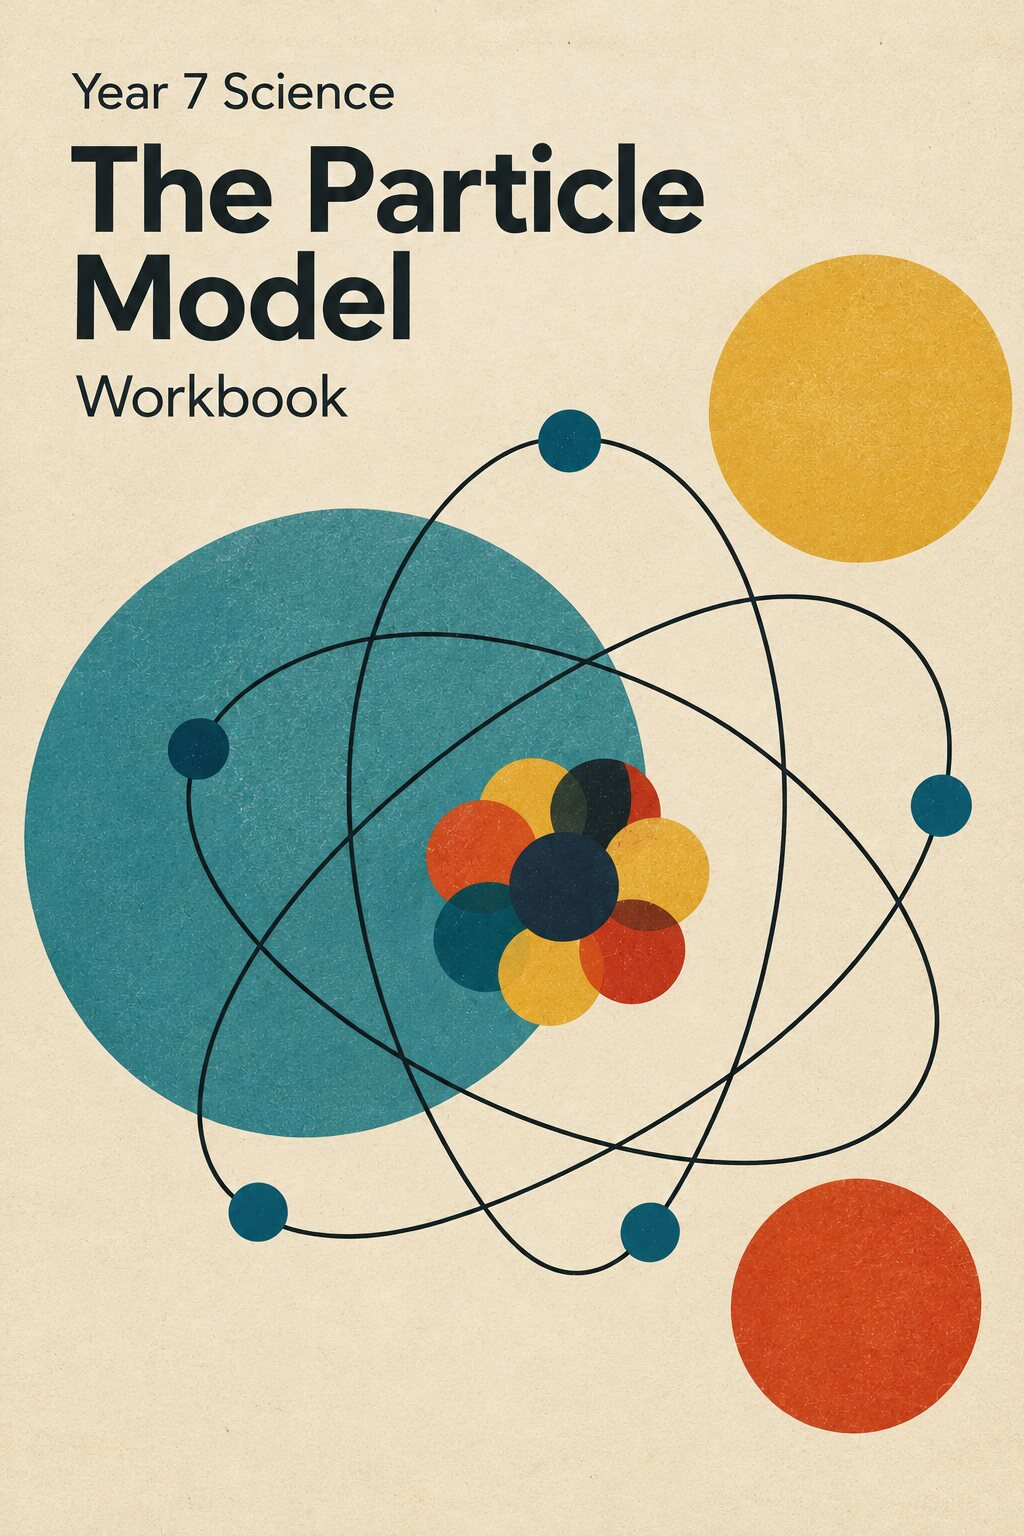
\includegraphics[width=\paperwidth]{../../../covers/particle-model.jpg}};
  \node[anchor=north east, fill=white, draw=Ink, line width=0.6pt, rounded corners=1.2mm,
        inner xsep=2mm, inner ysep=1.8mm, text width=30mm, font=\headingfont\footnotesize]
    at ([xshift=-4mm, yshift=-4mm]current page.north east)
    {\textbf{Name}\par\vspace{4mm}\hrule\vspace{2mm}\textbf{Class}\par\vspace{4mm}\hrule};
  \node[anchor=south east, fill=white, draw=Ink, line width=0.6pt, rounded corners=1.2mm,
        inner xsep=2.6mm, inner ysep=2mm, font=\headingfont\bfseries, align=right]
    at ([xshift=-4mm, yshift=6mm]current page.south east)
    {Advanced Particle Model 1\\[-1pt]{\normalfont\headingfont\scriptsize Topics 1--3}};
\end{tikzpicture}
\mbox{}
\clearpage

% ---- Inside cover ---------------------------------------------------------
\thispagestyle{plain}
{\headingfont\bfseries\fontsize{22}{26}\selectfont Advanced Particle Model}\par\vspace{1mm}
{\headingfont\large Book 1 \textbullet\ Topics 1--3 \textbullet\ Above the Year 7 level}\par\vspace{1mm}
{\small\itshape VC 2.0: VC2S8U05 \textbullet\ VC2S10U14 \textbullet\ VC2S10U15}\par\vspace{4mm}
\textbf{Teacher}\ \hrulefill\par

\begin{countrybox}{Acknowledgement of Country}
This booklet was created on the unceded Country of the Wurundjeri Woi-wurrung people of the Kulin Nation. We acknowledge Elders past, present and emerging.
\end{countrybox}

\begin{infobox}{How this booklet works}
\textbf{Advanced Particle Model} goes deeper into the ideas of the lesson books: more powerful models, the reasoning behind them, and harder problems that bring several ideas together. Each topic builds on the lessons named under its title. Each opens with its key vocabulary, then:\par\smallskip
\renewcommand{\arraystretch}{1.25}
\begin{tabular}{@{}p{24mm}p{70mm}@{}}
\textbf{Part A} & a reading with comprehension questions \\
\textbf{Part B} & the deeper idea, worked through \\
\textbf{Part C} & practice on your own \\
\textbf{Part D} & a challenge that pulls the ideas together \\
\end{tabular}

\smallskip
\begin{tabular}{@{}p{24mm}p{70mm}@{}}
\textbf{I do} \tagicon{\icodots{1}} & a worked example (solid frame) \\
\textbf{We do} \tagicon{\icodots{2}} & you try one with help (dashed frame) \\
\textbf{Reading} \tagicon{\icoread} & a passage to read (thin frame) \\
\end{tabular}
\end{infobox}

\clearpage
\markboth{Contents}{Contents}
{\headingfont\bfseries\LARGE Contents}\par\vspace{1mm}\noindent\rule{\linewidth}{0.6pt}\par\vspace{2mm}
\renewcommand{\arraystretch}{1.45}
\begin{tabular}{|C{1.1cm}|L{5.2cm}|C{1.7cm}|C{1.4cm}|}
  \hline\thead{Topic} & \thead{Title} & \thead{Deepens lesson} & \thead{Page} \\ \hline
  1 & \hyperlink{lesson.1.1}{Strange States of Matter} & 1 & \hyperlink{lesson.1.1}{p.\ \pageref{sec:1}} \\ \hline
  2 & \hyperlink{lesson.2.1}{Models and Their Limits} & 2, 4 & \hyperlink{lesson.2.1}{p.\ \pageref{sec:2}} \\ \hline
  3 & \hyperlink{lesson.3.1}{Particles, Energy and Temperature} & 4 & \hyperlink{lesson.3.1}{p.\ \pageref{sec:3}} \\ \hline
  4 & \textit{Energy and Changes of State} & 5 & Book 2 \\ \hline
  5 & \textit{Gas Pressure} & 7 & Book 2 \\ \hline
  6 & \textit{Density, Floating and Buoyancy} & 8 & Book 2 \\ \hline
  --- & \hyperlink{glossary}{Glossary} & & \hyperlink{glossary}{\pageref{sec:glossary}} \\ \hline
\end{tabular}
\renewcommand{\arraystretch}{1}
\clearpage
\setcounter{section}{0}\renewcommand{\lessonart}{1}
\sectiondiv{Strange States of Matter}{Plasma \textbullet{} Glass and other amorphous solids \textbullet{} Fluids that change their minds \textbullet{} Deciding a state from evidence}\label{sec:1}
\lessoncodes{Deepens Lesson 1 \textbullet{} VC2S8U05 \textbullet{} VC2S10I06}

\vocabhead
\begin{ctab}
\begin{tabular}{|SW{3.4cm}|W{7.0cm}|}
  \hline\hd & \thead{Word} & \thead{Definition (copy from the slide)} \\ \hline
  & \scaf{\textbf{Plasma}\label{voc:plasma}} & \scaf{A gas so hot that its particles break apart into charged pieces; it glows and conducts electricity.} \\ \hline
  & \textbf{Amorphous solid}\label{voc:amorphous-solid} & \\ \hline
  & \textbf{Crystalline solid}\label{voc:crystalline-solid} & \\ \hline
  & \textbf{Viscosity}\label{voc:viscosity} & \\ \hline
  & \textbf{Non-Newtonian fluid}\label{voc:non-newtonian-fluid} & \\ \hline
\end{tabular}
\end{ctab}

\lessonpart{A}{Reading and comprehension}{Teal}\label{read:1}

\begin{readingbox}{Reading --- Not Quite Solid, Not Quite Liquid}
Solid, liquid and gas describe almost everything you meet. But the universe is stranger. The Sun and every other star are made of \textbf{plasma}: matter so hot that its particles have been torn into electrically charged pieces. Plasma glows and carries electricity. Most of the visible matter in the universe is plasma, which makes it, not solid, the most common state of all.

Even on Earth the three states have blurry edges. In salt, sugar and metals the particles are packed in neat, repeating rows: they are \textbf{crystalline solids}. Glass is different. Its particles are jumbled like a liquid's, but locked in place. Glass is an \textbf{amorphous solid}, a solid without an orderly pattern. It holds its shape and does not flow at room temperature, so it is a solid.

Liquids differ too. How thick or runny a liquid is, its resistance to flowing, is its \textbf{viscosity}. Honey has high viscosity; water has low viscosity. For most liquids the viscosity stays the same however hard you stir. But cornflour in water, called oobleck, gets thicker the harder you push it: it is a \textbf{non-Newtonian fluid}. Tomato sauce does the opposite and runs more easily once you shake it.
\end{readingbox}

\rcreset
\rcq{Why is plasma described as the most common state in the universe?}{2.5cm}
\rcq{How is glass different from salt, and why is it still called a solid?}{3cm}
\rcq{What is viscosity? Give one liquid with high and one with low viscosity.}{2.5cm}
\rcq{How do oobleck and tomato sauce behave differently when you push or shake them?}{2.5cm}

\lessonpart{B}{Theory and examples}{Blue}\label{theory:1}

\subsection{Deciding a State from Evidence}\label{sub:a1.1}

\begin{skillbox}{Four tests}
\textbf{Shape:} does it keep its own shape? \quad \textbf{Volume:} does it keep the same volume? \quad \textbf{Flow:} does it flow and take the shape of its container? \quad \textbf{Squash:} can it be compressed?\\
A solid passes the first two and fails the last two; a liquid keeps its volume, flows and cannot be squashed; a gas fails the first two, flows and can be squashed.
\end{skillbox}

\begin{workedex}{Honey}
Honey flows slowly into the shape of a jar, keeps its volume, and cannot be squashed.

\smallskip
It keeps its volume but not its shape, and it cannot be compressed, so honey is a \textbf{liquid}, one with a high viscosity. Flowing slowly does not make something a solid.
\end{workedex}

\begin{wedo}{Sand}
Dry sand can be poured from a bucket and takes the shape of the container. A student says sand must be a liquid. Use the four tests, and think about a single grain, to decide whether she is right.
\answerbox{5cm}
\end{wedo}

\subsection{Compressing a Gas, by Numbers}\label{sub:a1.2}

\begin{skillbox}{How many times smaller?}
\[ \text{times smaller} = \frac{\text{volume before}}{\text{volume after}} \]
Only gases can be squashed this much, because their particles are far apart with empty space between them.
\end{skillbox}

\begin{workedex}{A sealed syringe}
A sealed syringe holds 100\,mL of air. The plunger is pushed in until the air fills 25\,mL.

\smallskip
$100 \div 25 = 4$: the air is \textbf{4 times smaller}. The same number of particles now has a quarter of the space, so they are closer together and hit the walls more often.
\end{workedex}

\begin{wedo}{A gas bottle}
A barbecue gas bottle has a volume of 20\,L. The gas inside would fill about 4000\,L at normal air pressure. How many times smaller is it in the bottle? (In fact the gas is squashed so hard it turns into a liquid.)
\workbox{4cm}
\end{wedo}

\lessonpart{C}{Practice}{Amber}\label{prac:1}

\begin{keepext}
\needspace{10\baselineskip}
\task A scuba tank has a volume of 12\,L. The air inside it would fill 2400\,L if it were let out at normal air pressure.
\pt{a}How many times smaller is the volume of the air in the tank than it would be outside?
\workbox{2.0cm}
\pt{b}Explain why you could not squash 2400\,L of \emph{water} into the same tank.
\answerbox{2.0cm}
\end{keepext}

\begin{keepext}
\needspace{10\baselineskip}
\task Cornflour mixed with a little water (``oobleck'') flows slowly when you tilt the bowl, but if you punch it quickly it feels hard and does not splash.
\pt{a}Give one property that suggests it is a liquid and one that suggests it is a solid.
\answerbox{2.0cm}
\pt{b}Explain why a scientist would say a single test is not enough to decide its state.
\answerbox{2.2cm}
\end{keepext}

\begin{keepext}
\needspace{10\baselineskip}
\task There is a fourth state of matter called \emph{plasma}. It is a gas so hot that it glows and conducts electricity. Lightning, the Sun and the inside of a neon sign are plasma. Is plasma matter? Use the two tests for matter in your answer.
\answerbox{2.8cm}
\end{keepext}

\begin{keepext}
\needspace{9cm}
\task Some people claim that old church windows are thicker at the bottom because glass is really a very slow liquid that has flowed down over hundreds of years. Scientists have calculated that, at room temperature, glass would take far longer than the age of the universe to flow even a tiny amount. Glassmakers in the past also made panes that were uneven to begin with.
\pt{a}What does the scientists' calculation suggest about the claim?
\answerbox{2.0cm}
\pt{b}Suggest a better explanation for why the bottoms of the windows are thicker.
\answerbox{2.0cm}
\end{keepext}

\begin{keepext}
\needspace{10\baselineskip}
\task Air is invisible, so some people think it is ``nothing''. Describe an observation from everyday life that shows air takes up space, and one that shows it has mass or pushes on things.
\answerbox{3.0cm}
\end{keepext}


\lessonpart{D}{Challenge}{Violet}\label{ext:1}

\task A toy shop sells ``slime''. Plan an investigation to decide whether it behaves more like a solid or a liquid. Describe at least three tests, what you would do in each, and what result you would expect if it were a solid and if it were a liquid.
\answerbox{9cm}

\clearpage

% ══════════════════════════════════════════════════════════════════════════════
%  TOPIC 2 — MODELS AND THEIR LIMITS                     (deepens Lessons 2, 4)
%  The master's Lesson 6, whole.
% ══════════════════════════════════════════════════════════════════════════════
\setcounter{section}{1}\renewcommand{\lessonart}{6}
\sectiondiv{Models and Their Limits}{Common wrong ideas \textbullet{} Fixing a particle explanation \textbullet{} Checking a particle diagram \textbullet{} What the model cannot show}\label{sec:2}
\lessoncodes{Deepens Lessons 2 and 4 \textbullet{} VC2S8U05 \textbullet{} VC2S8H01}

\vocabhead
\begin{ctab}
\begin{tabular}{|SW{2.91cm}|W{8.05cm}|}
  \hd & \thead{Word} & \thead{Definition (copy from the slide)} \\ \hline
  & \scaf{\textbf{Misconception}\label{voc:misconception}} & \scaf{An idea that many people believe but that is not correct.} \\ \hline
  & \textbf{Limitation}\label{voc:limitation} & \\ \hline
  & \textbf{Scale}\label{voc:scale} & \\ \hline
  & \textbf{Substance}\label{voc:substance} & \\ \hline
  & \textbf{Property}\label{voc:property} & \\ \hline
  & \textbf{Accurate}\label{voc:accurate} & \\ \hline
\end{tabular}
\end{ctab}

% ─── PART A ───────────────────────────────────────────────────────────────────
\lessonpart{A}{Reading and comprehension}{Teal}\label{read:6}

\begin{readingbox}{Reading --- What the Model Does Not Say}
The particle model is one of the most successful ideas in science, but it is easy to use it wrongly. A \textbf{misconception} is an idea that lots of people believe but that is not correct, and the particle model has some famous ones.

The biggest is the idea that particles are just tiny pieces of the \textbf{substance}, with all the same \textbf{properties}. When ice melts, the particles do not melt --- they stay exactly the same, and only their arrangement and movement change. When a metal rod gets longer as it heats up, the particles do not get bigger --- they move further apart. A single particle of copper is not orange, and a single particle of water is not wet. Colour, wetness, hardness and temperature are properties of huge numbers of particles together, not of one particle.

Another misconception is that there is air between the particles of a substance. There is nothing at all: just empty space. Air is made of particles too, so it cannot fill the gaps between particles.

Every model also has a \textbf{limitation}: something it cannot show, or shows in a way that is not \textbf{accurate}. Particle diagrams are drawn flat, with particles as coloured circles, and they are not to \textbf{scale}. In a real gas the particles are about ten times further apart than most diagrams show. Knowing a model's limitations is part of using it well.
\end{readingbox}

\rcreset
\rcq{What is a misconception?}{1.4cm}
\rcq{What happens to the particles of ice when the ice melts?}{1.6cm}
\rcq{When a metal rod gets longer as it is heated, what happens to its particles?}{1.6cm}
\rcq{Give two properties that the passage says belong to huge numbers of particles, not to one particle.}{1.6cm}
\rcq{What is between the particles of a substance? Why can it not be air?}{1.8cm}
\rcq{What is a limitation of a model?}{1.4cm}
\rcq{Give two ways particle diagrams are not accurate.}{1.8cm}
\rcq{Why is knowing a model's limitations part of using it well?}{1.8cm}

% ─── PART B ───────────────────────────────────────────────────────────────────
\lessonpart{B}{Theory and examples}{Blue}\label{theory:6}

\subsection{Common Wrong Ideas}\label{sub:6.1}

\begin{ctab}
\begin{tabular}{|L{4.53cm}|L{6.43cm}|}
  \thead{Wrong idea} & \thead{What the particle model really says} \\ \hline
  Particles melt, freeze or boil. & Particles stay the same. Their arrangement and movement change. \\ \hline
  Particles get bigger when heated. & Particles stay the same size. They move further apart. \\ \hline
  There is air between particles. & There is empty space --- nothing at all. \\ \hline
  Particles in a solid are not moving. & They vibrate all the time, even in the coldest solid. \\ \hline
  One particle has a colour or a temperature. & Colour and temperature belong to huge numbers of particles together. \\ \hline
  Liquid particles are spread out. & Liquid particles are close together, almost as close as in a solid. \\ \hline
\end{tabular}
\end{ctab}

\subsection{Fixing a Particle Explanation}\label{sub:6.2}

\begin{workedex}{Fixing an explanation}
A student writes: ``Butter melts in the sun because its particles melt.'' Find the mistake and write a correct explanation.

\medskip
\textbf{Mistake:} particles do not melt. They stay the same.

\textbf{Correct explanation:} the sun heats the butter, so its particles gain energy and vibrate faster. They break free of their fixed places and start to slide past each other, so the butter becomes a liquid.
\end{workedex}

\begin{wedo}{Fixing an explanation}
A student writes: ``A balloon gets bigger in the sun because the air particles inside it expand.'' Find the mistake and write a correct explanation.
\pt{a}The mistake.
\answerbox{1.6cm}
\pt{b}A correct explanation.
\answerbox{2.4cm}
\end{wedo}

\subsection{Checking a Particle Diagram}\label{sub:6.3}

\begin{skillbox}{Three rules for particle diagrams}
\begin{enumerate}[itemsep=1pt, leftmargin=1.4em, topsep=1pt]
  \item The particles of one substance are \textbf{the same size} in every state.
  \item Solid and liquid particles are \textbf{touching}; only the solid has a regular pattern.
  \item Gas particles are \textbf{far apart} and spread through the whole container.
\end{enumerate}
\end{skillbox}

\begin{workedex}{Checking a diagram}
This diagram is meant to show liquid water. What is wrong with it?

\begin{center}\pboxfig{\foreach \x/\y in {0.4/0.3,1.2/0.35,2.1/0.3,0.8/0.9,1.7/0.95,0.35/1.45,1.3/1.5,2.2/1.4}{\node[pA] at (\x,\y) {};}}{}\end{center}

\textbf{Mistake:} the particles are spread out with big gaps, like a gas.

\textbf{Fix:} liquid particles should be close together and touching, with no regular pattern.
\end{workedex}

\begin{wedo}{Checking a diagram}
This pair of diagrams is meant to show the same substance as a solid and as a gas. What is wrong with them?
\par\smallskip
\begin{center}\pboxfig{\stateIn{solid}{pB}}{solid}\hspace{4mm}\pboxfig{\foreach \x/\y in \gaspos{\node[pB, minimum size=6mm] at (\x,\y) {};}}{gas}\end{center}
\answerbox{3.6cm}
\end{wedo}

\subsection{What the Model Cannot Show}\label{sub:6.4}

\begin{workedex}{A limitation}
Give one limitation of drawing particles as coloured circles on a flat page.

\medskip
Real particles are \textbf{not coloured}, and they are arranged in three dimensions, not flat. A drawing also cannot show that the particles are moving all the time.
\end{workedex}

\begin{wedo}{A limitation}
A teacher uses marbles in a tray to model a solid, a liquid and a gas. Give one way the marbles are a good model of particles, and one limitation.
\pt{a}A way it is a good model.
\answerbox{1.8cm}
\pt{b}A limitation.
\answerbox{1.8cm}
\end{wedo}

% ─── PART C ───────────────────────────────────────────────────────────────────
\lessonpart{C}{Practice}{Amber}\label{prac:6}

Work through every task. For each wrong idea, say what is wrong and what is really happening.

\needspace{12\baselineskip}
\task Write \textbf{TRUE} or \textbf{FALSE} for each statement.

\vspace{4pt}
\begin{ctab}
\begin{tabular}{|SW{8.44cm}|Z{2.52cm}|}
  \hd & \thead{Statement} & \thead{True or false?} \\ \hline
  & A particle of gold is gold-coloured. & \scaf{FALSE} \\ \hline
  & The particles in an ice block are vibrating. & \\ \hline
  & There is air between the particles of water. & \\ \hline
  & When water boils, its particles move further apart. & \\ \hline
  & Particles get bigger when they are heated. & \\ \hline
\end{tabular}
\end{ctab}

\needspace{10\baselineskip}
\task A student writes: ``The chocolate went hard in the fridge because its particles froze.'' Rewrite the explanation so it is correct.
\answerbox{2.8cm}

\needspace{10\baselineskip}
\task A student writes: ``Railway tracks get longer on hot days because the metal particles grow.'' Rewrite the explanation so it is correct.
\answerbox{2.8cm}

\needspace{16\baselineskip}
\task Each diagram has one mistake. Describe it.

\vspace{4pt}
\begin{center}
\pboxfig{\foreach \r in {0,...,2}{\foreach \c in {0,...,6}{\node[pA] at (0.31+\c*0.33,0.2+\r*0.55) {};}}}{A: a solid}\hspace{1.4cm}%
\pboxfig{\foreach \x/\y in {0.5/0.3,1.3/0.32,2.1/0.3,0.9/0.7,1.75/0.72}{\node[pA] at (\x,\y) {};}}{B: a gas}
\end{center}
\begin{ctab}
\begin{tabular}{|SW{5.48cm}|W{5.48cm}|}
  \hd & \thead{Mistake in A} & \thead{Mistake in B} \\ \hline
  & & \\ \hline
\end{tabular}
\end{ctab}

\taskpair{Give one thing the particle model explains well.}{2.4cm}
         {Give one limitation of particle diagrams.}{2.4cm}

\needspace{10\baselineskip}
\task Explain why a single particle of water cannot be described as wet, even though water is wet.
\answerbox{2.6cm}

% ─── PART D ───────────────────────────────────────────────────────────────────
\needspace{14\baselineskip}\par\medskip{\headingfont\bfseries\large More practice}\par\smallskip
\begin{keepext}
\needspace{10\baselineskip}
\task Two groups build different models of the same mystery box. Both models explain all their observations.
\pt{a}Explain how both models could be ``right''.
\answerbox{2.2cm}
\pt{b}Describe a new test that could show which model is better.
\answerbox{2.2cm}
\end{keepext}

\begin{keepext}
\needspace{10\baselineskip}
\task A weather forecast predicts a 90\% chance of rain, but it stays dry all day. Does this mean the forecasting model is wrong? Explain your thinking.
\answerbox{2.8cm}
\end{keepext}

\begin{keepext}
\needspace{10\baselineskip}
\task Democritus's idea was not accepted for about two thousand years, but it is accepted today. What is needed before scientists accept a new model? Use the words \emph{evidence} and \emph{prediction}.
\answerbox{2.8cm}
\end{keepext}

\begin{keepext}
\needspace{10\baselineskip}
\task Scientists can never open up an atom and look inside, yet they are confident about what is in it. Explain how this is like the mystery box activity, and how it is different.
\answerbox{3.0cm}
\end{keepext}

\lessonpart{D}{Challenge}{Violet}
\begin{keepext}
\needspace{10\baselineskip}
\task Design a better model of a gas using students in the school hall. Describe what each student would do, and explain one thing your model shows well and one limitation it still has.
\answerbox{3.4cm}
\end{keepext}

\begin{keepext}
\needspace{10\baselineskip}
\task Water is unusual: ice floats on liquid water, so its particles must be slightly \emph{further apart} in the solid than in the liquid. Does this mean the three rules for particle diagrams are wrong? Explain how a scientist would handle an exception like this.
\answerbox{3.2cm}
\end{keepext}

\begin{keepext}
\needspace{10\baselineskip}
\task In air, particles are about ten particle-widths apart. If you drew a gas diagram to scale with particles 3\,mm wide, how far apart would you need to draw them? Would a gas diagram drawn this way fit in a 2.6\,cm box with eight particles? Explain.
\workbox{3.0cm}
\end{keepext}

\begin{keepext}
\needspace{10\baselineskip}
\task ``Temperature is how fast the particles are moving on average.'' Explain why the words \emph{on average} matter. What would you expect to find if you could measure the speed of every particle in a glass of water?
\answerbox{3.0cm}
\end{keepext}


\clearpage

% ══════════════════════════════════════════════════════════════════════════════
%  TOPIC 3 — PARTICLES, ENERGY AND TEMPERATURE               (deepens Lesson 4)
% ══════════════════════════════════════════════════════════════════════════════
\setcounter{section}{2}\renewcommand{\lessonart}{4}
\sectiondiv{Particles, Energy and Temperature}{Proof that particles exist \textbullet{} Temperature and kinetic energy \textbullet{} Absolute zero and kelvin \textbullet{} How heat moves}\label{sec:3}
\lessoncodes{Deepens Lesson 4 \textbullet{} VC2S8U05 \textbullet{} VC2S10U14}

\vocabhead
\begin{ctab}
\begin{tabular}{|SW{3.4cm}|W{7.0cm}|}
  \hline\hd & \thead{Word} & \thead{Definition (copy from the slide)} \\ \hline
  & \scaf{\textbf{Kinetic energy}\label{voc:kinetic-energy}} & \scaf{The energy an object or particle has because it is moving.} \\ \hline
  & \textbf{Brownian motion}\label{voc:brownian-motion} & \\ \hline
  & \textbf{Absolute zero}\label{voc:absolute-zero} & \\ \hline
  & \textbf{Kelvin}\label{voc:kelvin} & \\ \hline
  & \textbf{Thermal equilibrium}\label{voc:thermal-equilibrium} & \\ \hline
\end{tabular}
\end{ctab}

\lessonpart{A}{Reading and comprehension}{Teal}\label{read:3}

\begin{readingbox}{Reading --- The Dance of the Pollen Grains}
In 1827 the botanist Robert Brown watched tiny grains from inside pollen floating in water under his microscope. They jiggled about constantly, in random zigzags, and never stopped. This is now called \textbf{Brownian motion}. For almost eighty years nobody could explain it.

In 1905 Albert Einstein did. The grains, he said, are being struck from every side by water particles far too small to see. At any moment slightly more particles hit one side than the other, so the grain is shoved one way, then another. Einstein used the particle model to predict how far a grain should wander in a given time. In 1908 Jean Perrin measured it, and the numbers matched. Many scientists who had doubted that particles were real changed their minds.

Particles that move have \textbf{kinetic energy}. Temperature is a measure of the average kinetic energy of the particles: the hotter a substance, the faster its particles move. Cool something down and its particles slow. At \textbf{absolute zero}, about $-273$\,\textdegree C, they would have the least energy possible. Scientists measure from there using the \textbf{kelvin} scale, which starts at absolute zero.
\end{readingbox}

\rcreset
\rcq{What did Brown see, and why could he not explain it?}{2.5cm}
\rcq{Explain, in your own words, Einstein's explanation of Brownian motion.}{3cm}
\rcq{Why did Perrin's measurements change scientists' minds?}{2.5cm}
\rcq{What does temperature measure, in terms of particles?}{2cm}

\lessonpart{B}{Theory and examples}{Blue}\label{theory:3}

\subsection{The Kelvin Scale}\label{sub:a3.1}

\begin{skillbox}{Celsius and kelvin}
\[ \text{temperature in K} = \text{temperature in \textdegree C} + 273 \]
A change of 1\,\textdegree C is the same size as a change of 1\,K. There are no negative temperatures on the kelvin scale.
\end{skillbox}

\begin{workedex}{Converting}
Room temperature, 25\,\textdegree C: $25 + 273 = \mathbf{298\,K}$.\\
Liquid nitrogen boils at $-196$\,\textdegree C: $-196 + 273 = \mathbf{77\,K}$.
\end{workedex}

\begin{wedo}{Converting}
Convert to kelvin: water boiling (100\,\textdegree C); a freezer ($-18$\,\textdegree C). Convert to \textdegree C: 0\,K; the surface of the Sun, about 5800\,K.
\workbox{4.5cm}
\end{wedo}

\subsection{How Heat Moves}\label{sub:a3.2}

\begin{workedex}{A cold spoon in hot tea}
Explain, with particles, why a cold spoon left in hot tea warms up and the tea cools.

\smallskip
The tea's particles move fast and collide with the spoon's slower particles, making them vibrate faster. Each collision passes on some kinetic energy, so the spoon's particles speed up and the tea's slow down. Energy keeps moving from hot to cold until both are the same temperature. They are then in \textbf{thermal equilibrium}, and there is no more overall flow of energy.
\end{workedex}

\begin{wedo}{An ice cube in a drink}
Use particles to explain what happens to the ice cube and to the drink when an ice cube is dropped into a glass of water at room temperature. When does the change stop?
\answerbox{5cm}
\end{wedo}

\lessonpart{C}{Practice}{Amber}\label{prac:3}

\begin{keepext}
\needspace{10\baselineskip}
\task A balloon full of air is cooled in a freezer and shrinks a little. Use the particle model to suggest why. (Hint: think about how fast the particles move and how hard they hit the inside of the balloon.)
\answerbox{3.0cm}
\end{keepext}

\begin{keepext}
\needspace{10\baselineskip}
\task In air, the particles are on average about ten particle-widths apart. Particle diagrams of gases usually show them only two or three widths apart.
\pt{a}Why do you think diagrams are drawn this way?
\answerbox{2.0cm}
\pt{b}What wrong idea could this give someone?
\answerbox{2.0cm}
\end{keepext}

\begin{keepext}
\needspace{10\baselineskip}
\task Glass is a solid, but its particles are not arranged in a regular pattern. Does this break the particle model? Explain what glass tells us about how a solid is defined.
\answerbox{3.0cm}
\end{keepext}

\begin{keepext}
\needspace{10\baselineskip}
\task A drop of water contains about 1\,700\,000\,000\,000\,000\,000\,000 particles. If you could count one particle every second, without stopping, roughly how many years would it take to count them all? There are about 32 million seconds in a year. Show your working.
\workbox{3.0cm}
\end{keepext}
\begin{keepext}
\needspace{10\baselineskip}
\task Bigger grains in water jiggle less than tiny grains. Use the particle model to suggest why.
\answerbox{2.8cm}
\end{keepext}

\begin{keepext}
\needspace{10\baselineskip}
\task The coldest possible temperature is called \emph{absolute zero}, about $-273$\,\textdegree C. At absolute zero, particles would have the least possible kinetic energy.
\pt{a}Explain why nothing can be colder than absolute zero.
\answerbox{2.0cm}
\pt{b}The temperature in deep space is about $-270$\,\textdegree C. How many degrees above absolute zero is this?
\workbox{1.8cm}
\end{keepext}

\begin{keepext}
\needspace{10\baselineskip}
\task Brown at first wondered whether the pollen grains were moving because they were alive. To test this, he looked at grains of dust and crushed rock in water, and saw them jiggle in the same way. Explain what this test showed, and why it was a good test.
\answerbox{3.0cm}
\end{keepext}

\begin{keepext}
\needspace{10\baselineskip}
\task In a gas at room temperature, particles move at hundreds of metres per second --- faster than a passenger jet. Yet a smell takes a minute or more to cross a room. Use the idea of collisions to explain why.
\answerbox{3.2cm}
\end{keepext}


\lessonpart{D}{Challenge}{Violet}\label{ext:3}

\task A cup of water and a full bath are both at 40\,\textdegree C.
\pt{a} Compare the average kinetic energy of the particles in each.
\answerbox{3cm}
\pt{b} Which has more energy altogether? Explain.
\answerbox{3cm}
\pt{c} Which would melt more ice? Use your answers to explain why temperature and the total amount of thermal energy are not the same thing.
\answerbox{4cm}

\clearpage

% ══════════════════════════════════════════════════════════════════════════════
%  TOPIC 4 — ENERGY AND CHANGES OF STATE                     (deepens Lesson 5)
% ══════════════════════════════════════════════════════════════════════════════

\clearpage\markboth{Glossary}{Glossary}\hypertarget{glossary}{}\pdfbookmark[1]{Glossary}{glossarybm}
{\headingfont\bfseries\LARGE Glossary}\label{sec:glossary}\par\vspace{1mm}\noindent\rule{\linewidth}{0.6pt}\par
{\small Every key word in this booklet and the page it is introduced on.}\par\smallskip
\renewcommand{\arraystretch}{1.3}
\begin{longtable}{|>{\RaggedRight}p{34mm}|p{9mm}|p{\dimexpr\linewidth-43mm-6\tabcolsep-4\arrayrulewidth-1pt\relax}|}
\hline \rule{0pt}{4mm}\headingfont\bfseries Word & \headingfont\bfseries Page & \headingfont\bfseries In my own words \\ \hline \endhead
  Absolute zero & \pageref{voc:absolute-zero} & \\ \hline
  Accurate & \pageref{voc:accurate} & \\ \hline
  Amorphous solid & \pageref{voc:amorphous-solid} & \\ \hline
  Brownian motion & \pageref{voc:brownian-motion} & \\ \hline
  Crystalline solid & \pageref{voc:crystalline-solid} & \\ \hline
  Kelvin & \pageref{voc:kelvin} & \\ \hline
  Kinetic energy & \pageref{voc:kinetic-energy} & \\ \hline
  Limitation & \pageref{voc:limitation} & \\ \hline
  Misconception & \pageref{voc:misconception} & \\ \hline
  Non-Newtonian fluid & \pageref{voc:non-newtonian-fluid} & \\ \hline
  Plasma & \pageref{voc:plasma} & \\ \hline
  Property & \pageref{voc:property} & \\ \hline
  Scale & \pageref{voc:scale} & \\ \hline
  Substance & \pageref{voc:substance} & \\ \hline
  Thermal equilibrium & \pageref{voc:thermal-equilibrium} & \\ \hline
  Viscosity & \pageref{voc:viscosity} & \\ \hline
\end{longtable}
\padtofour
\end{document}
